%from chapin2013:  An individual bolometer acts as a thermal absorber which are linked directly to transition edge sensors.  When the sensors detect detect thermal variations they will produce changing currents which result in changing magnetic fields.  The magnetic fields are detected by super conduction quantum interference devices (SQUIDs) prior to the output currents being digitized.  Between the initial SQUID amplification and digitization of the current, the data is resampled from 12KHz to 200Hz.  A chain of ``dark SQUIDs'' is used to detect any non-thermal noise that can arise from the amplification of the signal.  //all unnecessary....
\chapter{Observations and Data Preparation}\label{observations}

\section{SCUBA-2} \\
The Submillimetre Common-User Bolometer Array 2 (SCUBA-2) was designed to decrease the observing time of the sub-millimeter sky relative to its predecessor SCUBA \citep{holland2013}.  This would benefit the community by allowing for rapid data acquisition in the submillimeter regime of the electromagnetic spectrum, at the 450$\mu$m and 850$\mu$m bands in particular.  Prior to SCUBA-2, other bolometer camera's such as LABOCA, BOLOCAM and SHARC-II were limited to less than 100 pixels, while the new SCUBA-2 has been able to incorporate over 10,000 pixels in its design and effectively reduce the required observing time \citep{chapin2013}.  Increasing the amount of pixels by a factor of 100 was possible by the advent of new technology such as high precision micromachining, superconducting transition edge sensors, and superconducting quantum interference device amplifiers (SQUIDs) \citep{holland2013}.

The observations of NGC3627 were taken from the Nearby Galaxies Legacy Survey's (NGLS) initial science images using SCUBA-2 from December 29, 2011  to January 21, 2012, and consist of 24 18$\arcmin$ by 18$\arcmin$ scans taken in grade 3 weather or better $(0.08 < \tau <0.12)$ with observations centered at 450$\mu$m and 850$\mu$m emission with a 32$\mu$m and 85$\mu$m bandpass respectively.  16 of the 24 scans were deemed useable, and whether or not an observation was deemed worthwhile was determined by factors such as the behavior of the image background or whether the image was flagged during observing to be unusable.  The observations of NGC3627 were taken using a daisy scanning pattern  to help remove any random noise by introducing crossing points.  The scanning speed of the JCMT was 150$\arcsec$/second in order to negate any drifting effects seen from the instrumentation \citep{chapin2013}.

\section{Image Creation and Properties}

For any imaging process to have be successful, the image need to have limited white noise \citep{chapin2013}.  White noise in the sense of our bolometer observations arise from thermal variations in the instrument and atmosphere during data acquisition. The random noise is minimized through scanning methods and during image processing \citep{chapin2013}.  To create the final SCUBA-2 data products we use the Submillimetre User Reduction Facility (SMURF) procedure MAKEMAP.  This procedure reduces the noise of the observations while maintaining the source's emission by incorporating a combination of principal component analysis and a maximum likelihood analysis \citep{chapin2013}.  Both of these methods have proven useful in reducing bolometer data on their own, but due to the size of raw SCUBA-2 data, either method on its own would result in extreme run times or the process becoming resource intensive \citep{chapin2013}.


MAKEMAP breaks down the image creation into several steps performed in iteration in order to successfully reduce any background noise \citep{chapin2013}.  The raw data is approximated by equation \ref{eq:sc2_raw} such that $b_i(t)$ is the i$^{th}$ bolometer output at time t, f is a scaling factor determined from flat field calibrations, $e_i(t)$ is the extinction at time t for the i$^{th}$ bolometer, $a_i(t)$ is the astronomical signal for i$^{th}$ bolometer at time t, noise from the product of the common mode and gain, $g_i*n_c(t)$, low-frequency noise $n_f(t)$ and random noise $n_r(t)$\citep{chapin2013}.

\begin{equation}\label{eq:sc2_raw}
  b_i(t) = f \left[ e_i(t)*a_i(t) + g_i*n_c(t)+n_f(t)+n_r(t)\right]
\end{equation}

The steps used in MAKEMAP are:  COM and GAI which estimate a common mode signal and from the fitting averaging time-series of each bolometer observation, EXT to apply the measured extinction corrections, FLT to apply a high- and low-pass filters to remove any noise features not removed in the COM and GAI filtering, AST which regrids the data and detects sources to be removed from reduction.  The final step is NOI which determines the noise in the gridded map after each step has been performed and is calculated by isolating the white noise component in equation \ref{eq:sc2_raw}.  A convergence check is then issued based on the magnitude of change in each pixel from the previous map and the current version.  If the check failed the COM, GAI, EXT, and FLT values are recalculated using the AST information obtained from the previous iteration, and the process is repeated until the convergene values are met or the maximum number of iterations have been carried out \citep{chapin2013}.

%MAKEMAP breaks down the image creation into several steps performed in iteration in order to successfully reduce any background noise \citep{chapin2013}.  The steps used in MAKEMAP are:  COM and GAI which remove any common noise features detected by the SQUIDs, EXT to apply extinction corrections, FLT to apply a high- and low-pass filters to remove any noise features not removed in the COM and GAI filtering, AST which regrids the data and detects sources to be removed from reduction.  The final step is NOI which determines the noise in the gridded map after each step has been performed.  A convergence check is then issued and if the check failed the COM, GAI, EXT, and FLT values are inverted and the process is repeated with the inverted values \citep{chapin2013}.
In our production of maps, we used the configuration file dimmconfig\_bright\_compact.lis and altered the AST and FLT sections of the image creation by introducing a mask made from Herschel's 250$\mu$m map.  The purpose of the mask was to exclude the target from interfering with the noise minimization as well as prohibit any emission from the galaxy to be significantly altered during image production.  The filter size of the high-pass filter was also modified, and an appropriate value was determined to be 175$\arcsec$.  We determined an appropriate high-pass filter size by running a large range of filters from 100$\arcsec$ to 300$\arcsec$ and inspecting the total recovered flux of NGC3627.  A plot of the returned flux values can be seen in figure \ref{fig:filt_lines}.  An good filter would not show any significant decrease flux compared to the 350$\mu$m or 500$\mu$m.  This requirement removes any filters greater than 200$\arcsec$.  Given the flux was nearly unchaning with filters less than 200$\arcsec$, we determiend an appropriate filter size by examining the structure that was returned in particular how well the spiral arms were effected for the 850$\mu$m, and how well the disk was preserved in the 450$\mu$m.  The spatial effect of the filters can be seen in figure \ref{fig:450_flt} for the 450$\mu$m and figure \ref{fig:850_flt} for the 850$\mu$m.  The maps were returned from MAKEMAP in units of pW with a pixel size of 2$\arcsec$ by 2$\arcsec$ for both the 450$\mu$m and 850$\mu$m.

\begin{figure}
  \centering
  \includegraphics[scale=0.65]{obs_imgs/flux_line.jpeg}
  \label{fig:filt_lines}
  \caption[Flux Values vs  High-Pass Filter Sizes]{Returned flux values for NGC3627 with varying high-pass filter sizes.}
\end{figure}

\begin{figure}
  \centering
  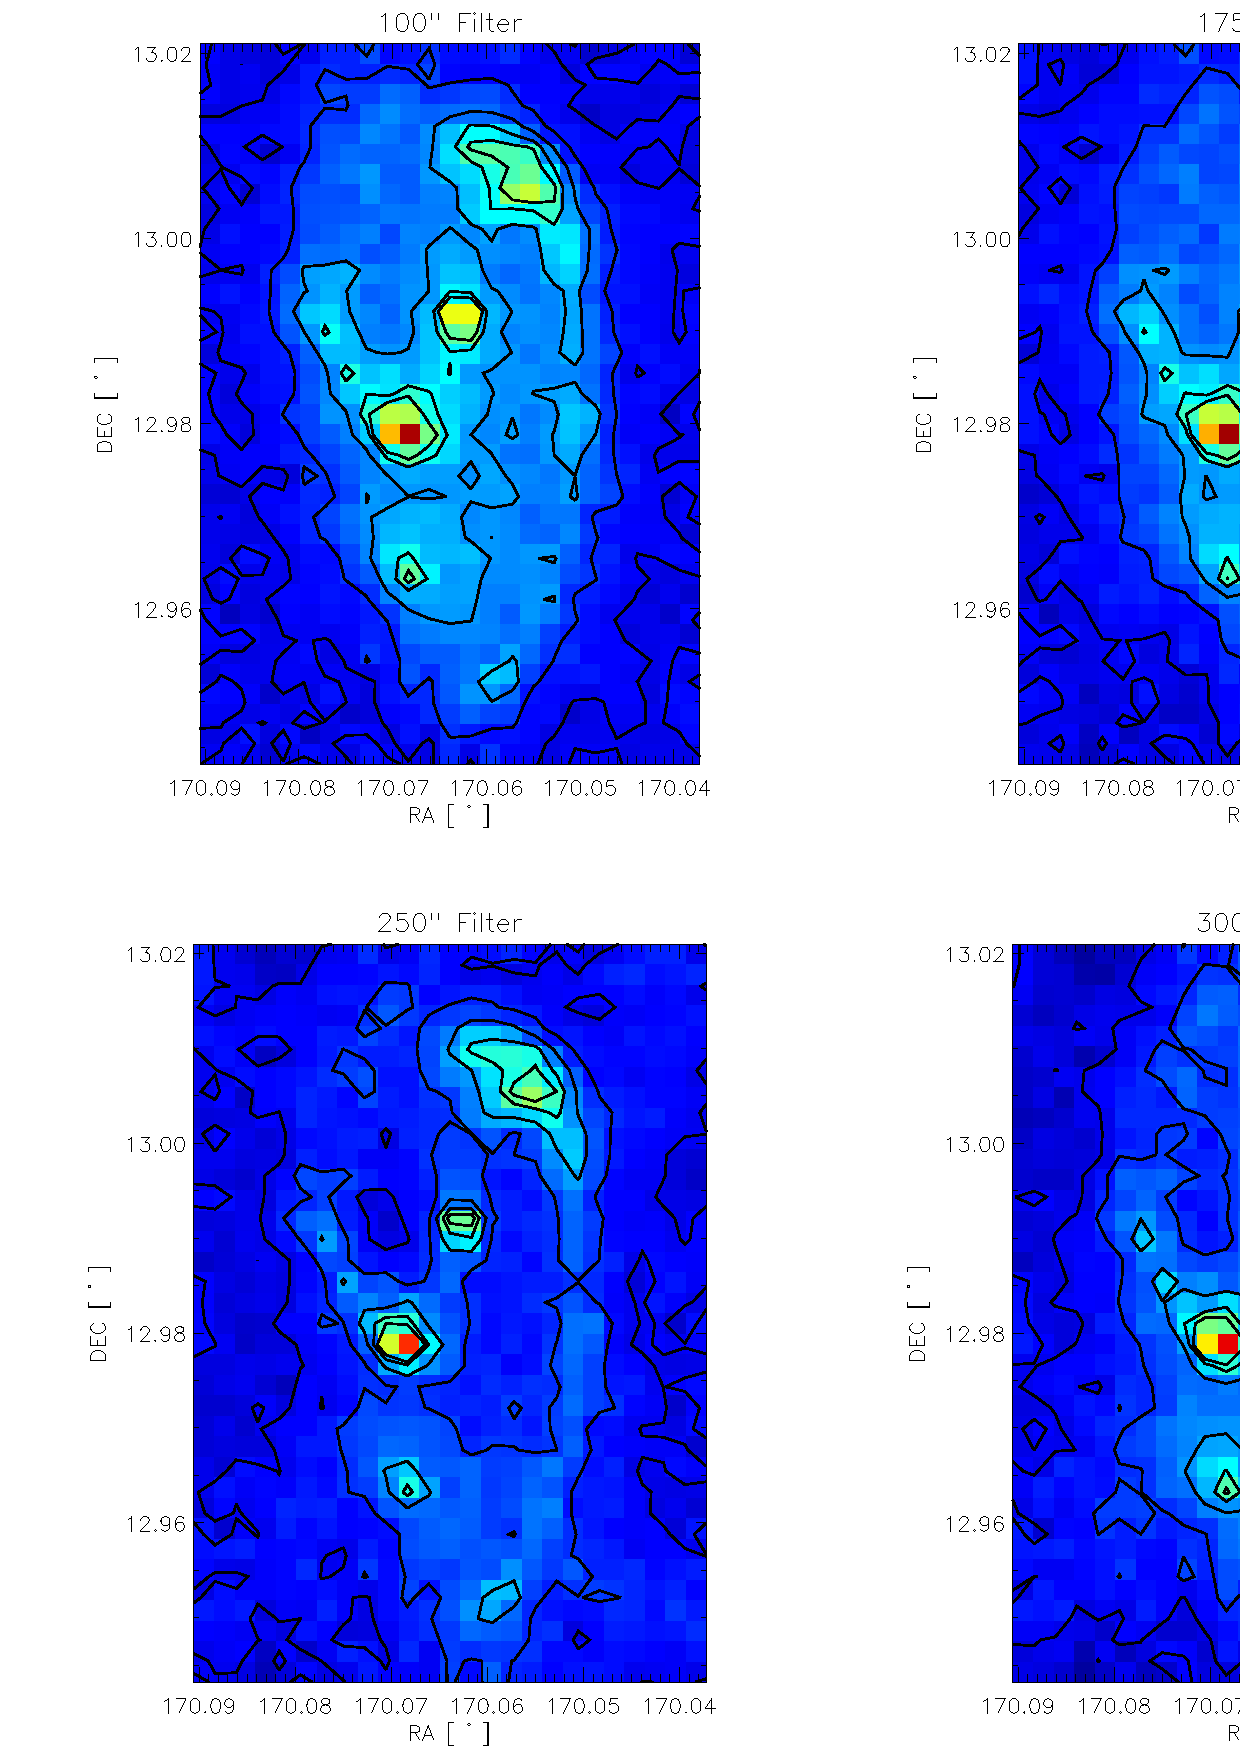
\includegraphics[scale=0.5]{obs_imgs/450_comparison_4.jpeg}
  \label{fig:450_flt}
  \caption[450$\mu$m High-Pass Filter Images]{Four 450$\mu$m maps of NGC3627 using varying high-pass filter sizes.  The contours shown are for 0.0, 0.02, 0.05, 0.08 and 0.1 Jy/pixel for each image.}
\end{figure}

\begin{figure}
  \centering
  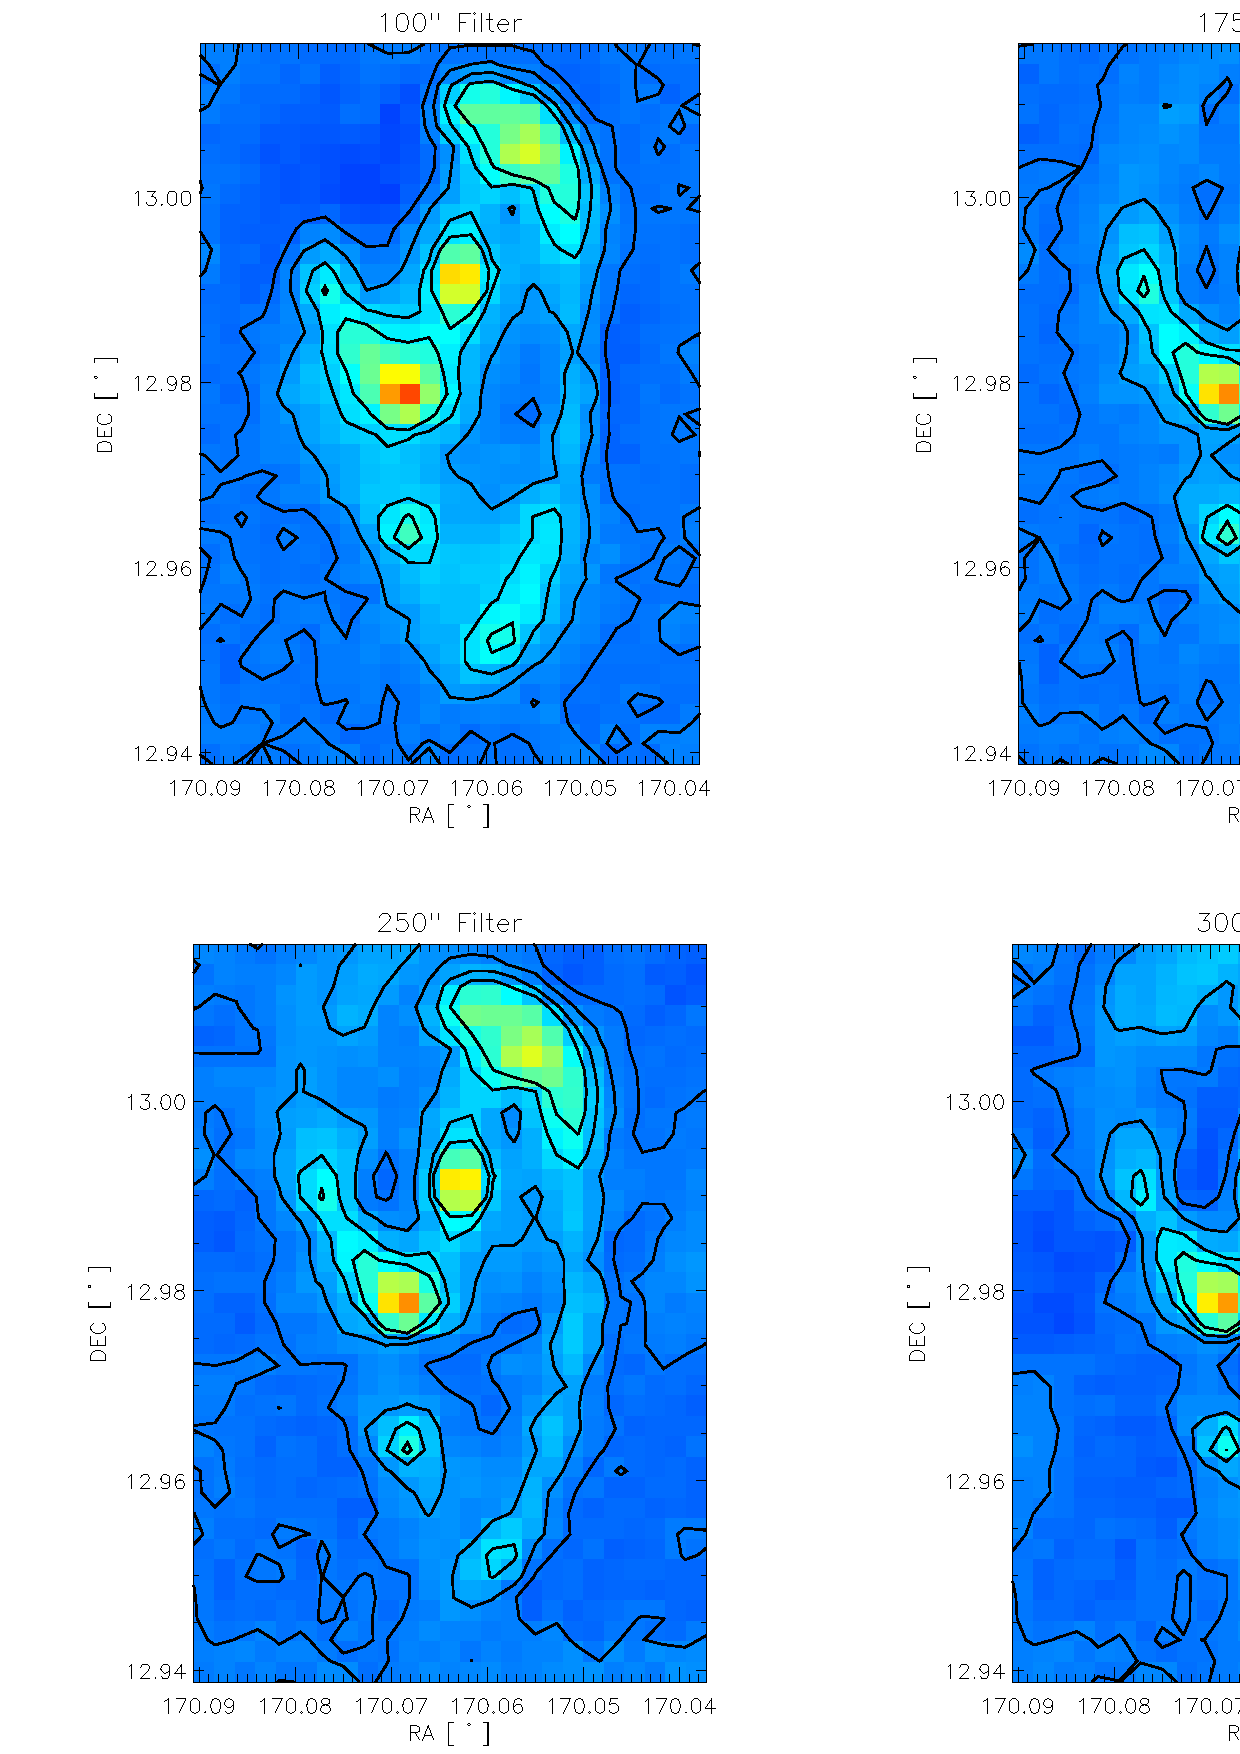
\includegraphics[scale=0.5]{obs_imgs/850_comparison_4.jpeg}
  \label{fig:850_flt}
  \caption[850$\mu$m High-Pass Filter Images]{Four 850$\mu$m maps of NGC3627 using varying high-pass filter sizes.  The contours shown are for 0.0, 0.002, 0.005, and 0.008 Jy/pixel for each image.}
\end{figure}

The finalized 450$\mu$m image was then re-gridded down to a 4$\arcsec$ by 4$\arcsec$ pixel grid, and flux calibration values of 491000 and 4710 were applied to convert from pW to mJy/beam and mJy/square arcsecond respectively.  The 850$\mu$m maps were re-gridded to an 8$\arcsec$ by 8$\arcsec$ pixel size and used flux calibration values of 537000 and 2340 for mJy/beam and mJy/square arcsecond.  The 4$\arcsec$  and 8$\arcsec$ pixels corresponed to a 180pc and 360pc size scale for our target, NGC3627.  To simplify the analysis, the images are also converted to Jy/pixel.  The 450$\mu$m and 850$\mu$m are shown in figures \ref{fig_450} and \ref{fig_850}.  The calibration values are determined from our calibrator source, Uranus.  The overall noise in the final image can be seen in table \ref{tab_obs_scuba2}.

\begin{figure}
  \centering
  \label{fig_450}
  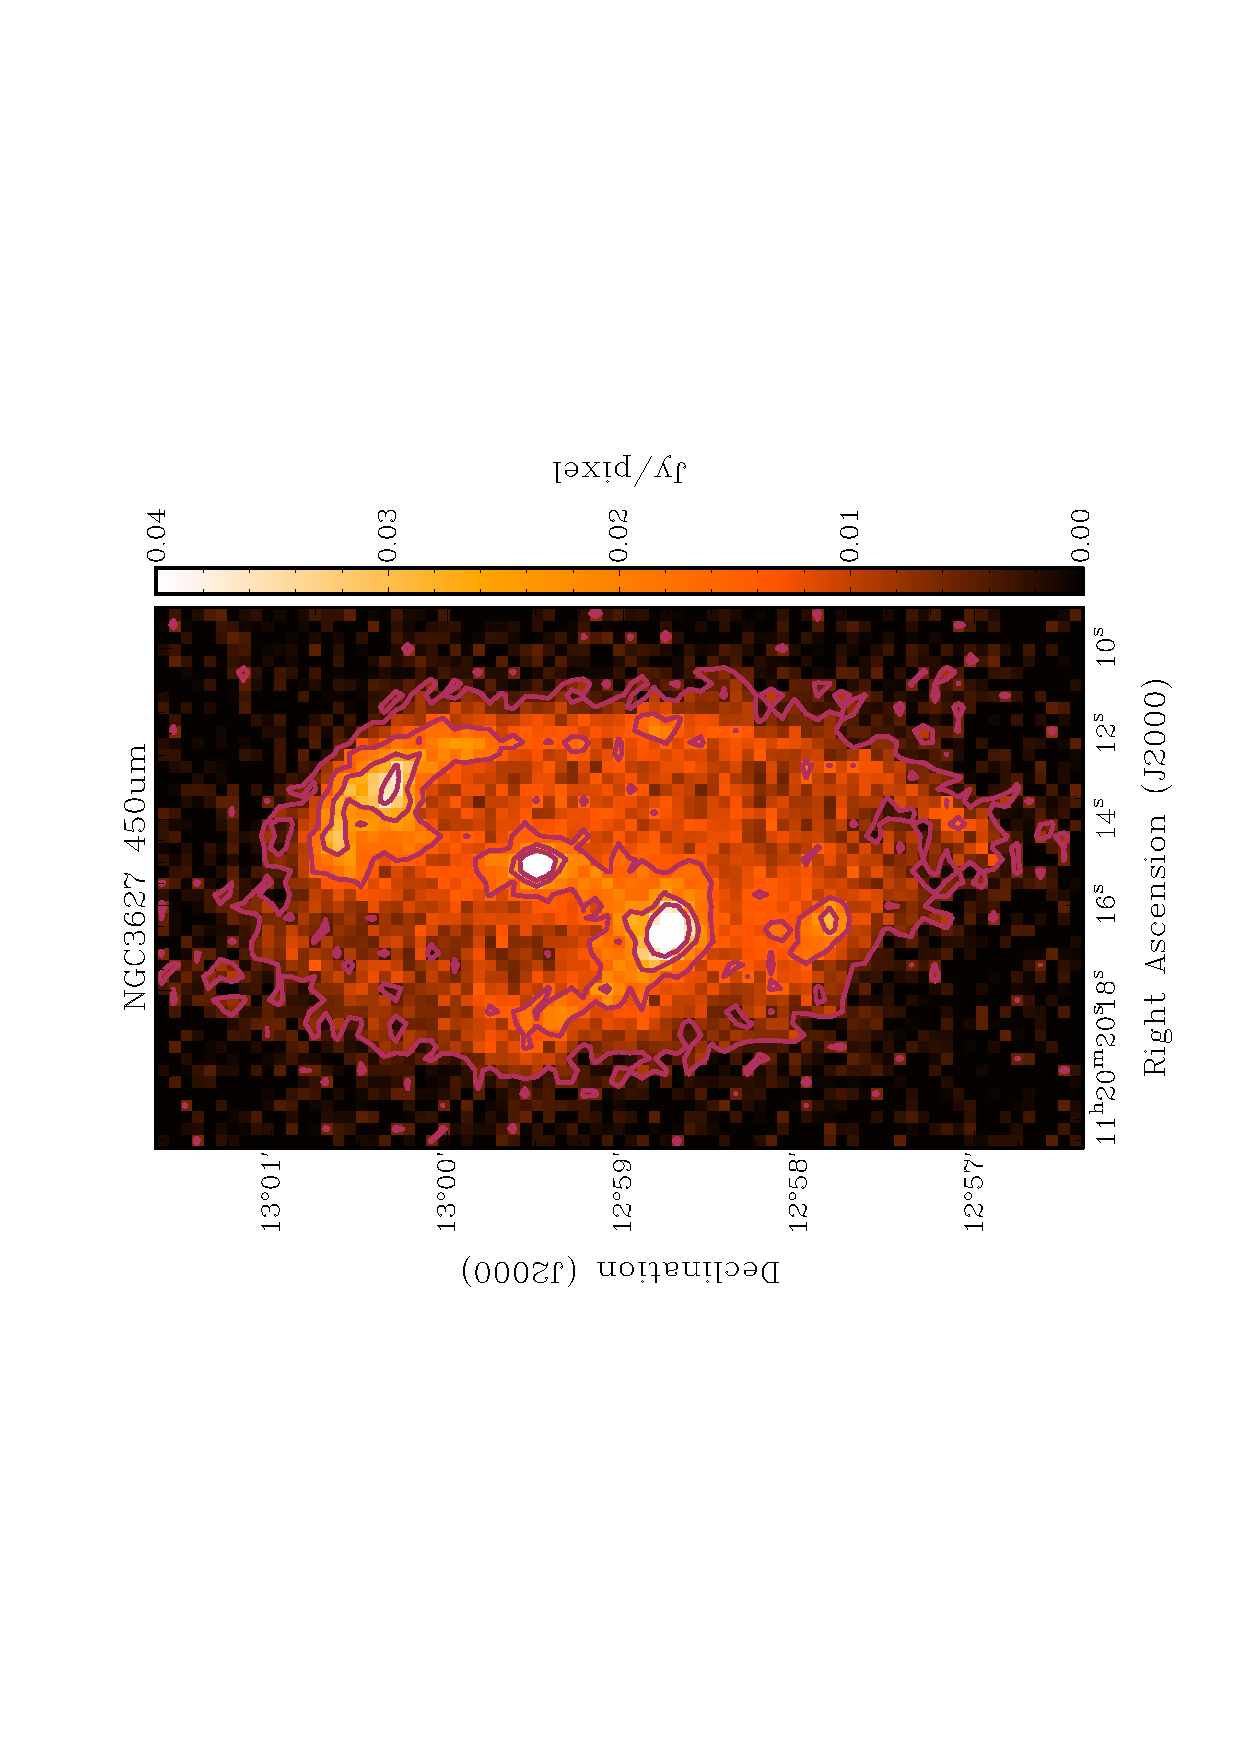
\includegraphics[scale=0.5,angle=270]{obs_imgs/450_um.jpeg}
  \caption[NGC3627 450$\mu$m Observations]{450$\mu$m observation produced at the end of the image production.}
\end{figure}

\begin{figure}
  \centering
  \label{fig_850}
  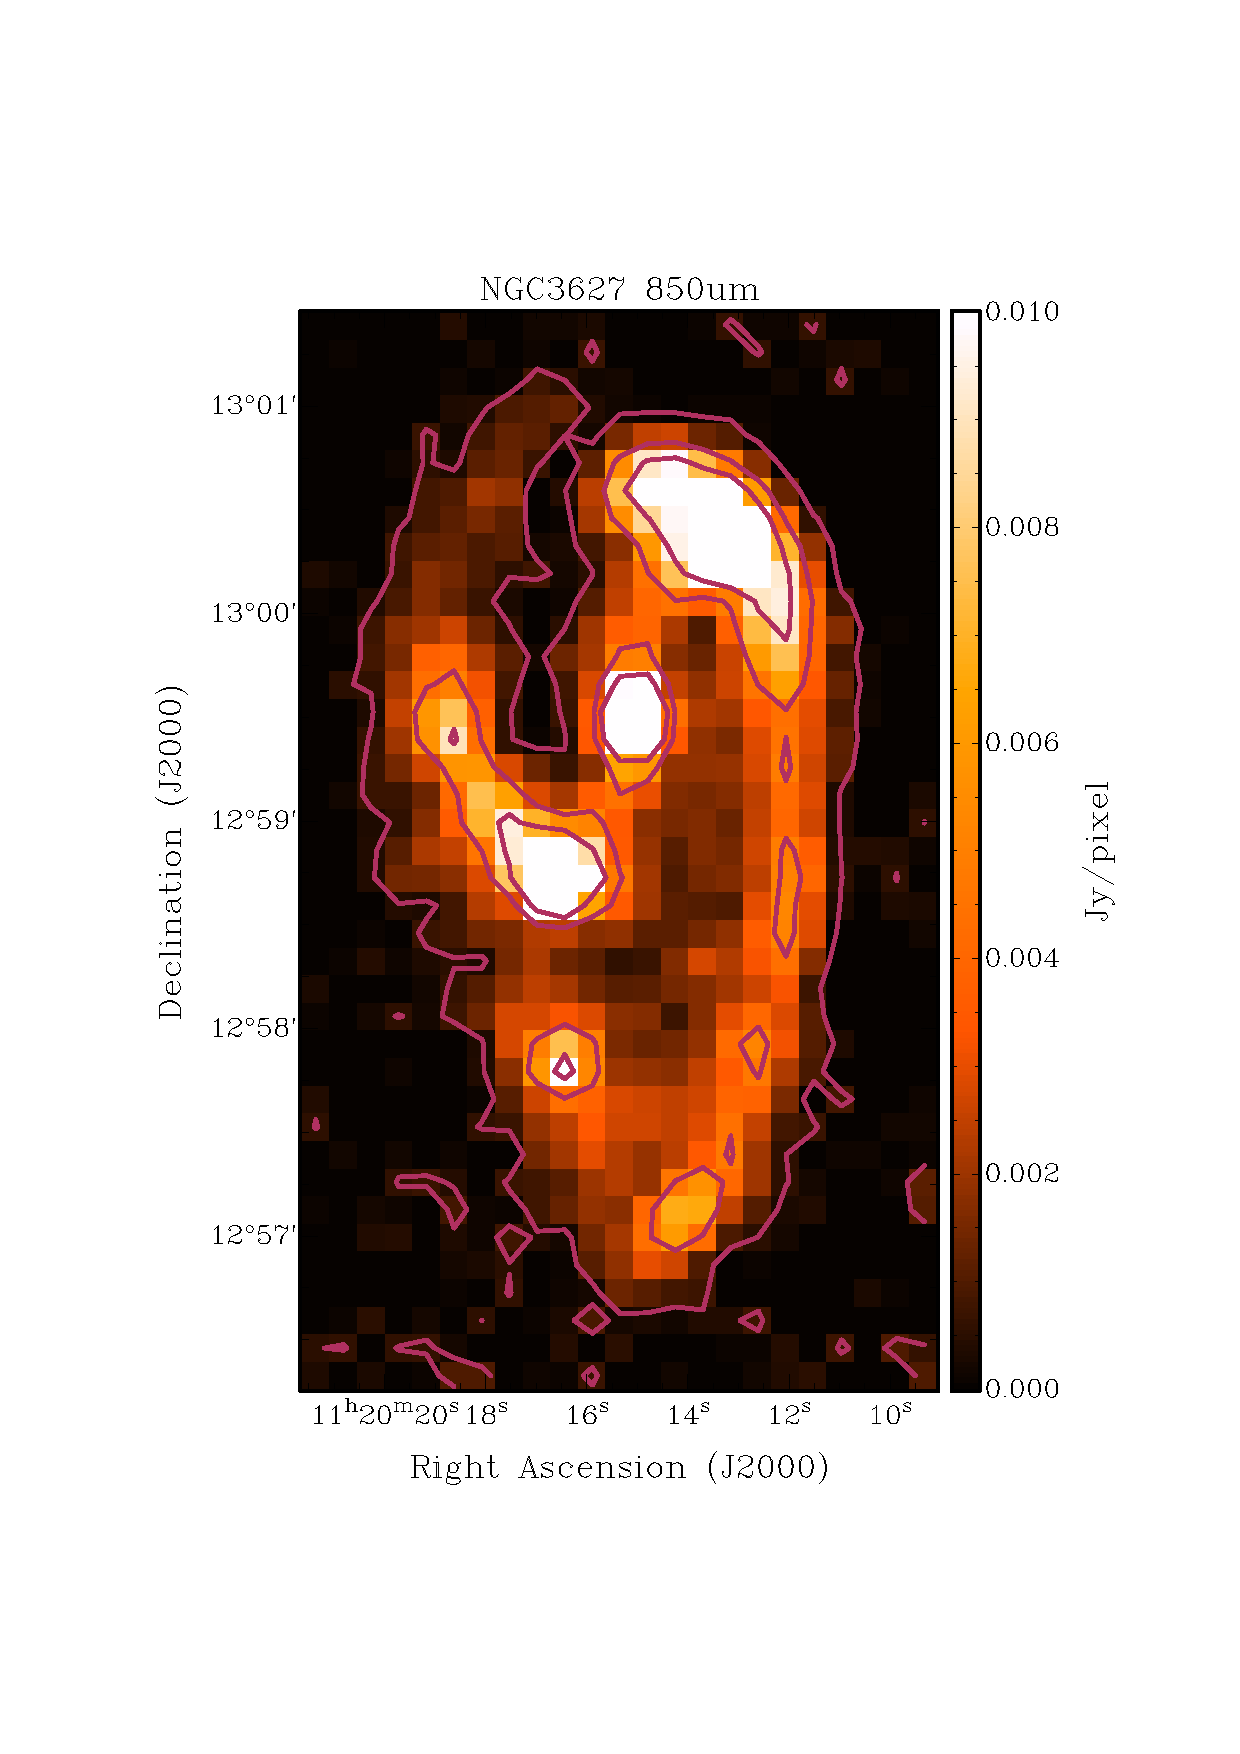
\includegraphics[scale=0.5]{obs_imgs/850_um.jpeg}
  \caption[NGC3627 850$\mu$m Observations]{850$\mu$m observation produced at the end of the image production.}
\end{figure}

\begin{deluxetable}{cccccc}
  \tabletypesize{\footnotesize}
  \tablecolumns{6}
  \tablewidth{0pt}
  \tablecaption{Properties of NGC3627 SCUBA-2 Observations\label{tab_obs_scuba2}}
  \tablehead{\colhead{Observation} & \multicolumn{4}{c}{Beam Properties} & \colhead{RMS} \\
& $\alpha$ & $\theta_{\alpha}$ & $\beta$ & $\theta_{\beta}$ & \it{[mJy / Pixel]}}
  \startdata
    450$\mu$m & 0.854 $\pm$ 0.002 & 7.48$\arcsec$ $\pm$ 0.03$\arcsec$ & 0.146 $\pm$ 0.003 & 23.1$\arcsec$ $\pm$ 0.2$\arcsec$ & 3.42  \\
    850$\mu$m & 0.9624 $\pm$ 0.0002 & 12.8$\arcsec$ $\pm$ 0.004$\arcsec$ & 0.0376 $\pm$ 0.0002 & 44.5$\arcsec$ $\pm$ 0.09$\arcsec$ &  0.476 \\
   \enddata
\end{deluxetable}

\subsection{Beam Shape of the 450$\mu$m and 850$\mu$m Data} \\
The Uranus calibration images were also used in determining the shape of the beam for the 450$\mu$m and 850$\mu$m observations.  The beam shape of both the 450$\mu$m and 850$\mu$m maps deviates from a single gaussian due to the second maximum of the airy diffraction pattern in the response function of the telescope and minor imperfections in the mirror of the JCMT due to boundaries of the panel \citet{dempsey2013}.  This abnormality was best represented by a sum of two gaussians whose amplitude totals to unity \citep{dempsey2013}.  The average beam resolution for the 450$\mu$m and 850$\mu$m are reported in table \ref{tab_obs_scuba2} and match the values within uncertainty found in \citep{dempsey2013}.  The calibration images and beams can be seen in figure \ref{fig_calib}.  The contribution of the error beam in the 850$\mu$m emission is negligible and allows the beam to be approximated by a single gaussian.  However, the contribution of the error beam in the 450$\mu$m images was large enough to require special treatment in order to properly match beams for analysis.

\begin{figure}
  \label{fig_calib}
  \centering
  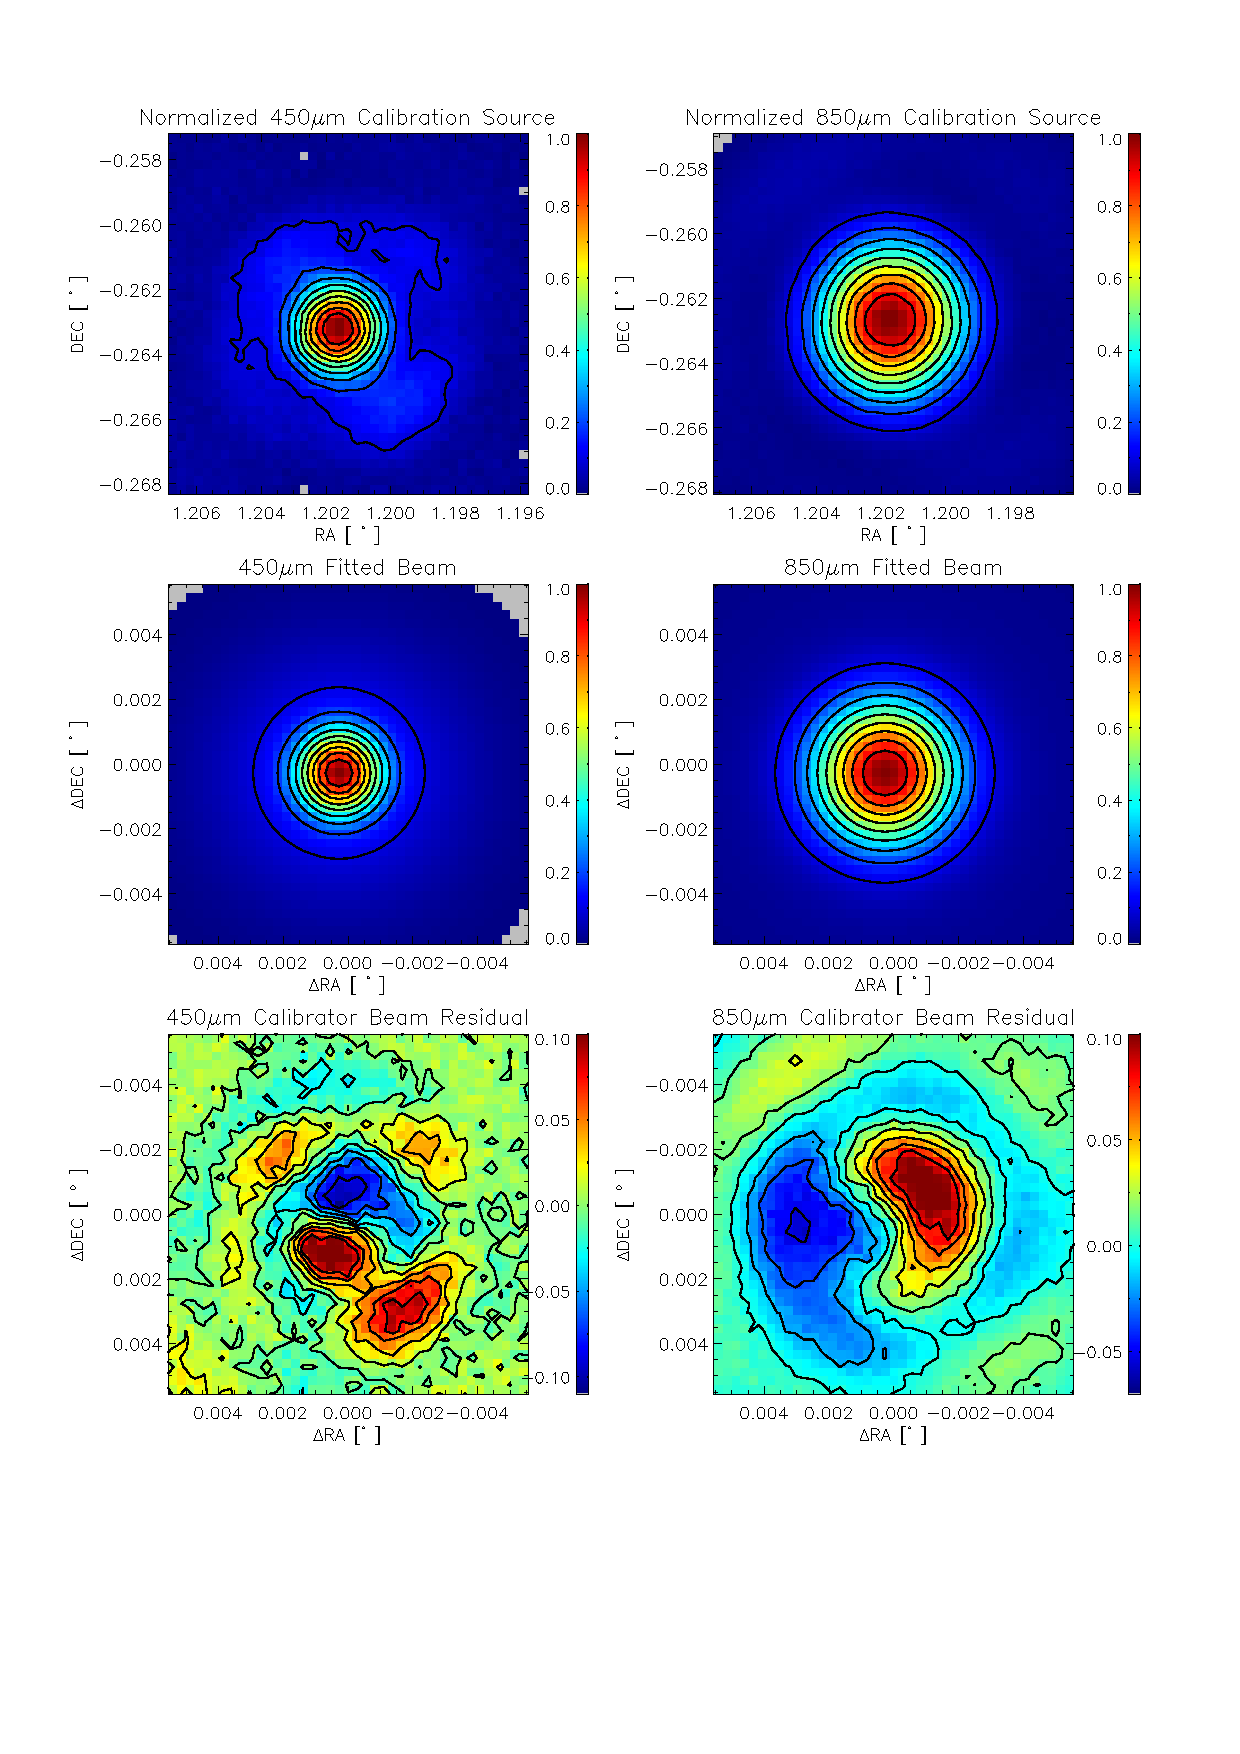
\includegraphics[scale=0.5]{obs_imgs/calib_beams.jpeg}
  \caption[SCUBA-2 Calibration and Beams]{The top row shows the Uranus images taken on January, 5th 2012 for the 450$\mu$m on the left and the 850$\mu$m on the right.  The bottom row shows the fitted beams for the 450$\mu$m on the right and 850$\mu$m on the left using the double gaussian beam shape.}
\end{figure}

\section{Ancillary Data}

The science goals of this thesis required data outside the capabilities of SCUBA-2.  For instance, accurately determining the dust mass involved fitting the spectral energy distribution (SED) for NGC3627.  To successfully fit an SED, we needed shorter wavelength data to fully probe the cold component of this galaxy. We used data ranging from 100$\mu$m to 500$\mu$m from the KINGFISH survey (\citep{kennicutt2011}) to gain a large enough wavelength range for fitting the cold component.  Secondly, the bandpass of the 850$\mu$m emisison contains the CO j=3-2 transmission line.  In order to get a valid approximation on the dust mass, this contribution had to be removed.  We used emission data from the NGLS using HARP instrumentation on the JCMT \citep{wilson2012}.  When a dust mass was obtained, we used CO j=1-0 from the Nobeyama 45-m telescope (\citep{kuno2007}), CO j=2-1 from HERACLES (\citep{leroy2009}), and $HI$ observations from THINGS (\citep{walter2008}) to determine an reasonable molecular hydrogen mass to calculate a dust-to-gas ratio.

\subsection{Key Insights on Nearby Galaxies: a Far-Infrared Survey with Herschel (KINGFISH)}

%sings paper not showing up

The Key Insights on Nearby Galaxies: a Far-Infrared Survey with Herschel (KINGSFISH) was designed to be a follow up to the Spitzer Infrared Nearby Galaxies Survey (SINGS) \citep{kennicutt2003} with observations of the warm and cold component of dust emission using the increased resolution from Herschel \citep{kennicutt2011}.  The main science goals of the KINGFISH survey were to better understand the star formation processes that were shielded by dust, resolved studies of heating and cooling of the interstellar medium (ISM), and to build an inventory of how cold dust emission relates to other dust components in the ISM \citep{kennicutt2011}.  The survey consisted of studying 61 nearby galaxies (d$<$30Mpc) that cover a range of environments each observed at 70$\mu$m, 100$\mu$m, 160$\mu$m, 250$\mu$m, 350$\mu$m, and 500$\mu$m.  Our analyis focuses on fitting the cold component of NGC3627's SED, so we omitted the 70$\mu$m emission from the fitting, and processed the data through MAKEMAP as described in $\S$ \ref{data_agree}.  The rms and beam size after the large scale structure has been removed can be seen in table \ref{tab_obs_kfish}, while the preconvolved maps are shown in figures \ref{fig_100} to \ref{fig_500}.

\begin{figure}
  \centering
  \label{fig_100}
  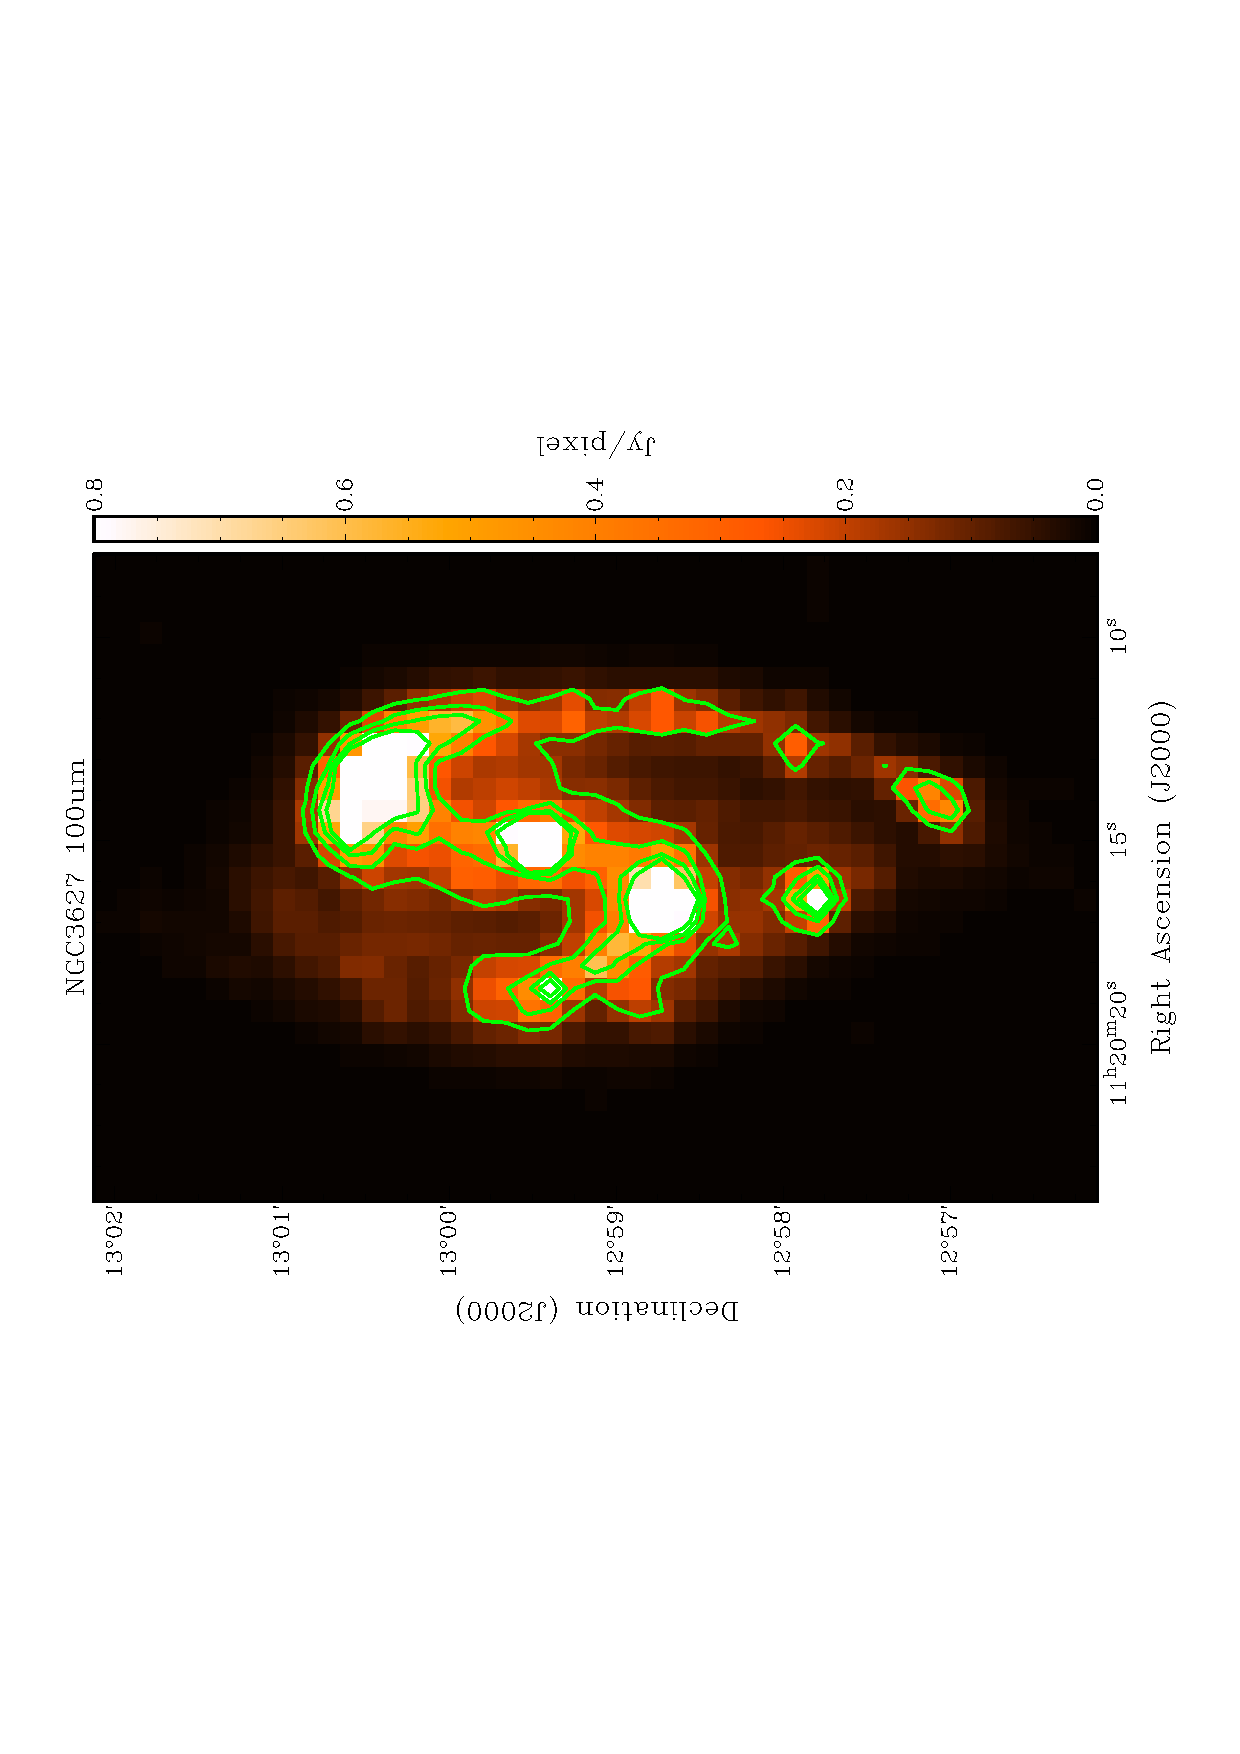
\includegraphics[scale=0.5,angle=270]{obs_imgs/100_um.jpeg}
  \caption[NGC3627 100$\mu$m Observations]{Residual of the MAKEMAP filtering of 100$\mu$m observations.}
\end{figure}

\begin{figure}
  \centering
  \label{fig_160}
  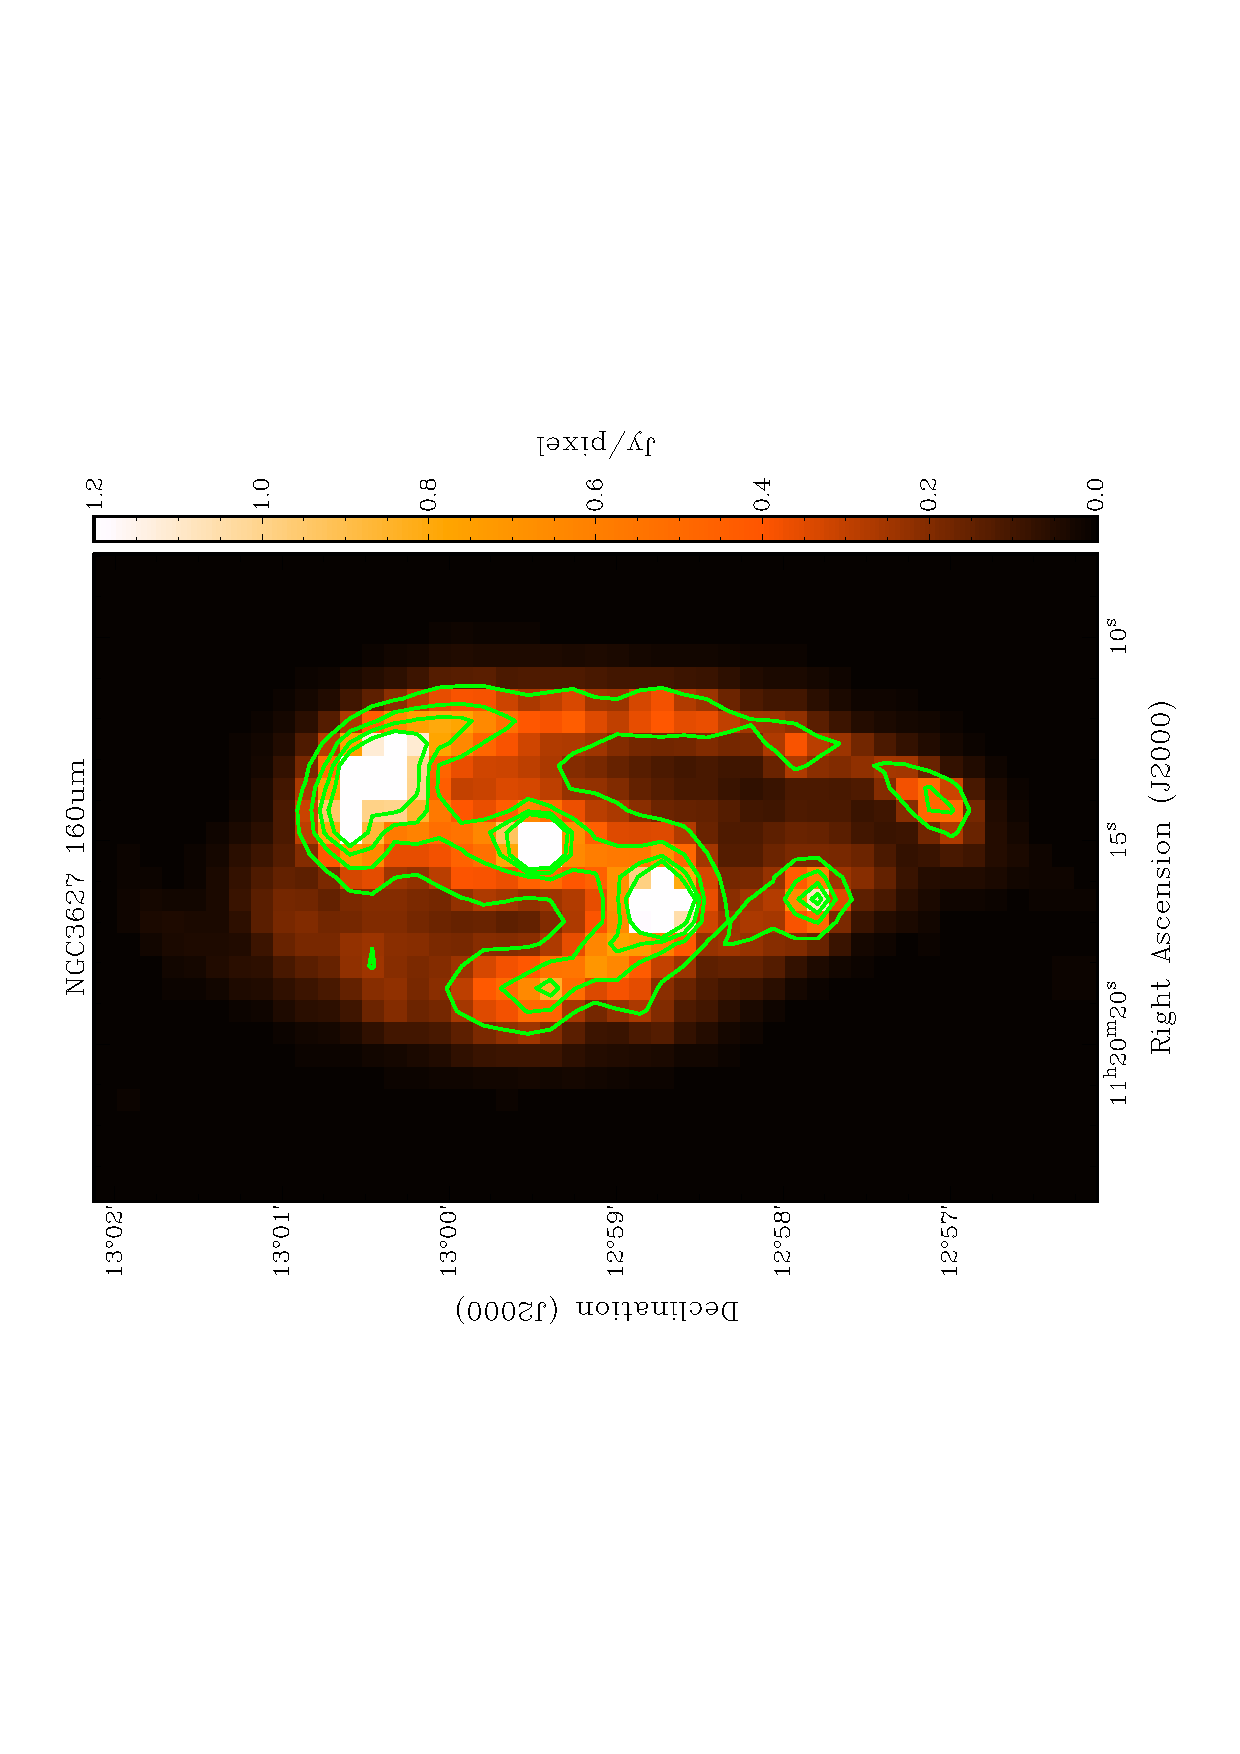
\includegraphics[scale=0.5,angle=270]{obs_imgs/160_um.jpeg}
  \caption[NGC3627 160$\mu$m Observations]{Residual of the MAKEMAP filtering of 160$\mu$m observations.}
\end{figure}

\begin{figure}
  \centering
  \label{fig_250}
  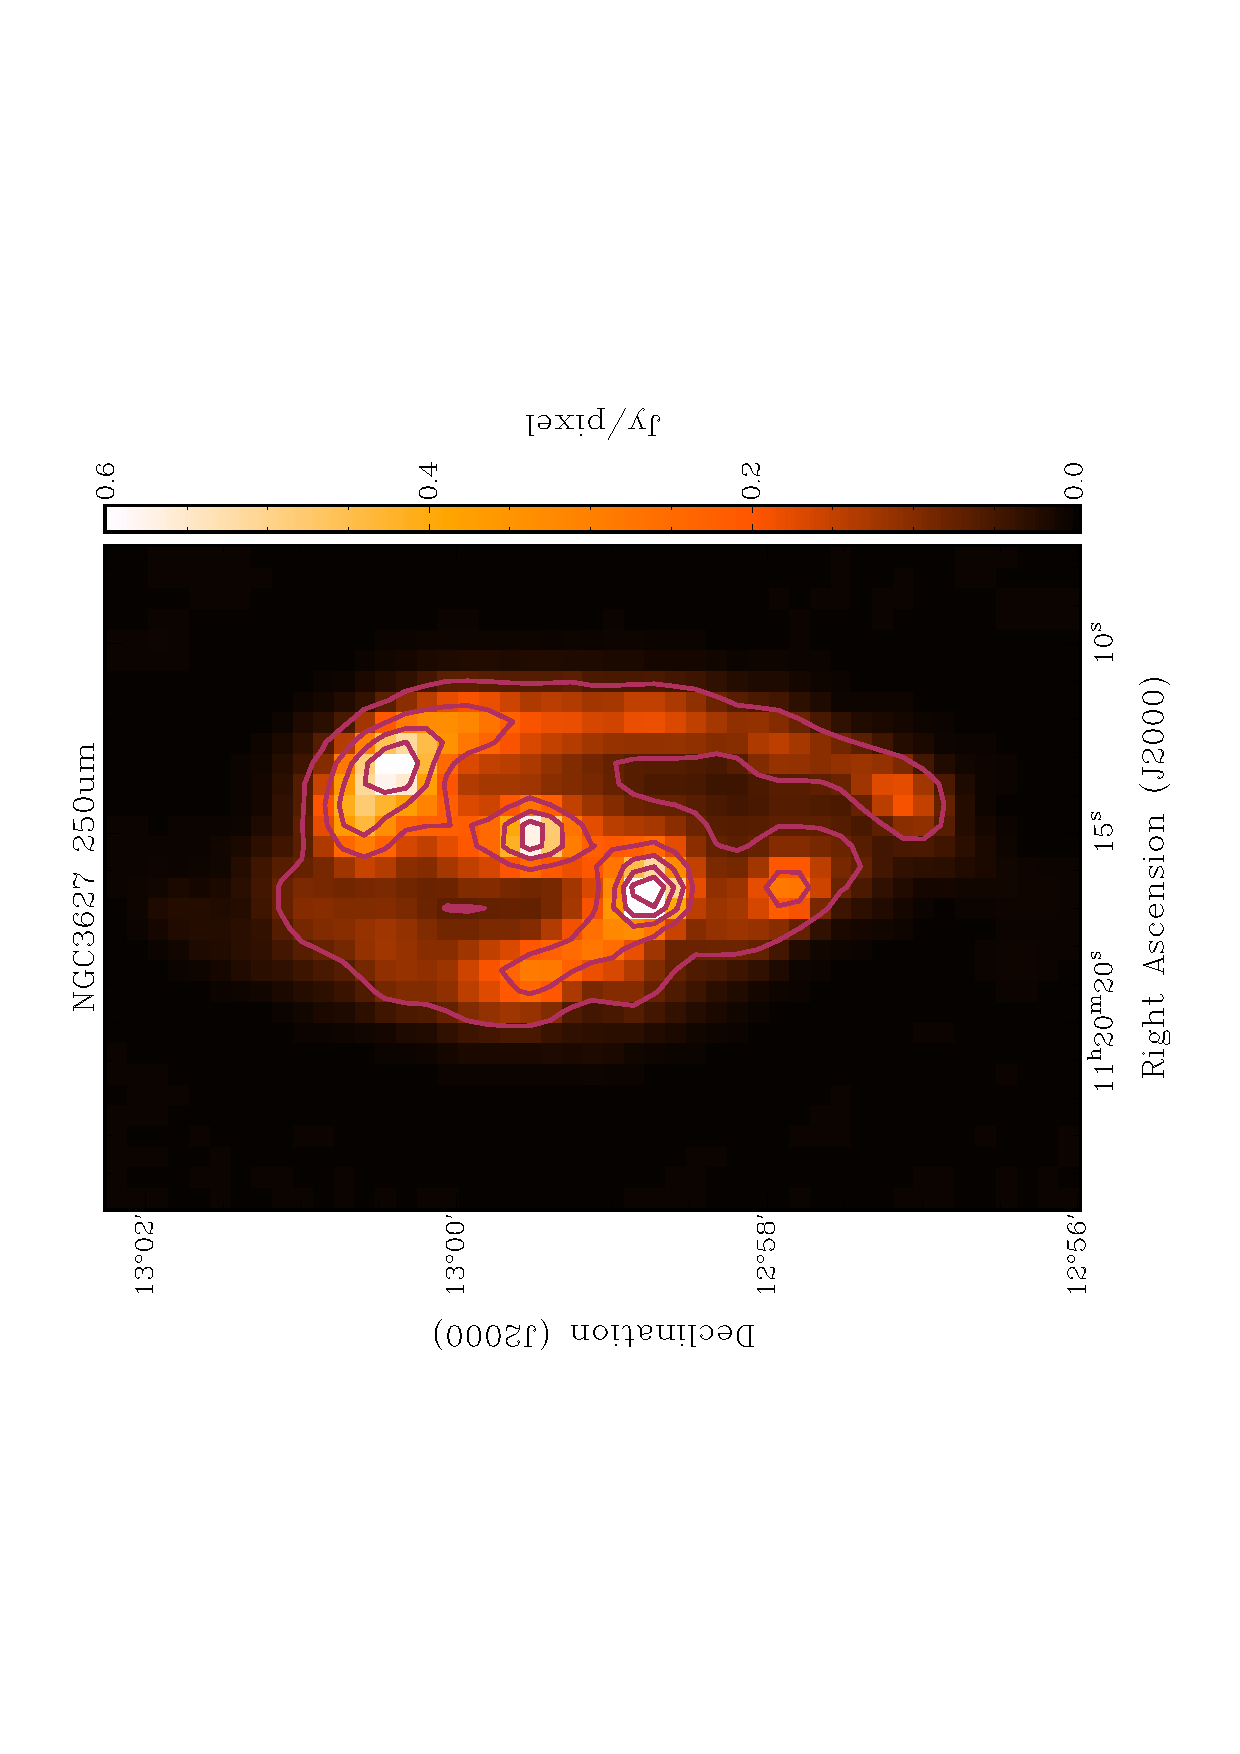
\includegraphics[scale=0.5,angle=270]{obs_imgs/250_um.jpeg}
  \caption[NGC3627 250$\mu$m Observations]{Residual of the MAKEMAP filtering of 250$\mu$m observations.}
\end{figure}

\begin{figure}
  \centering
  \label{fig_350}
  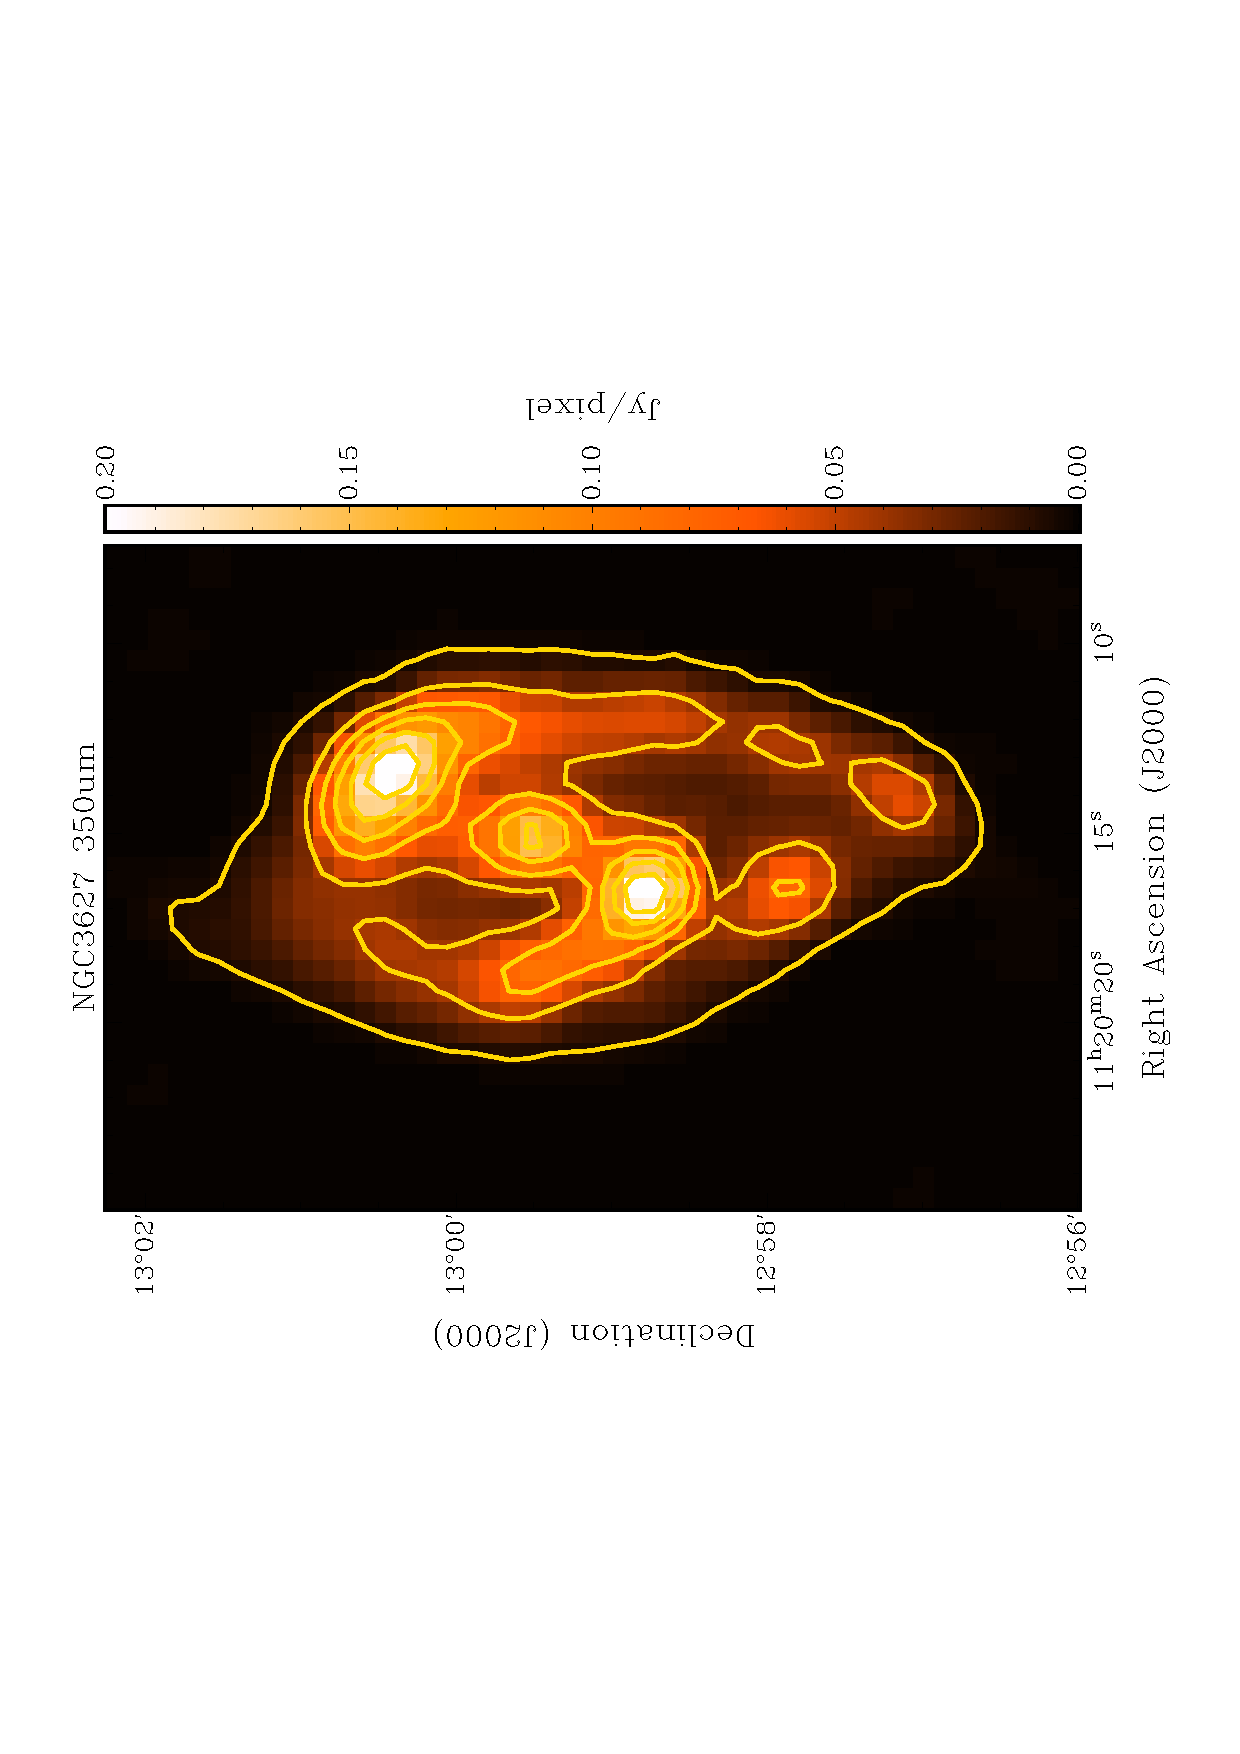
\includegraphics[scale=0.5,angle=270]{obs_imgs/350_um.jpeg}
  \caption[NGC3627 350$\mu$m Observations]{Residual of the MAKEMAP filtering of the 350$\mu$m observations.}
\end{figure}

\begin{figure}
  \centering
  \label{fig_500}
  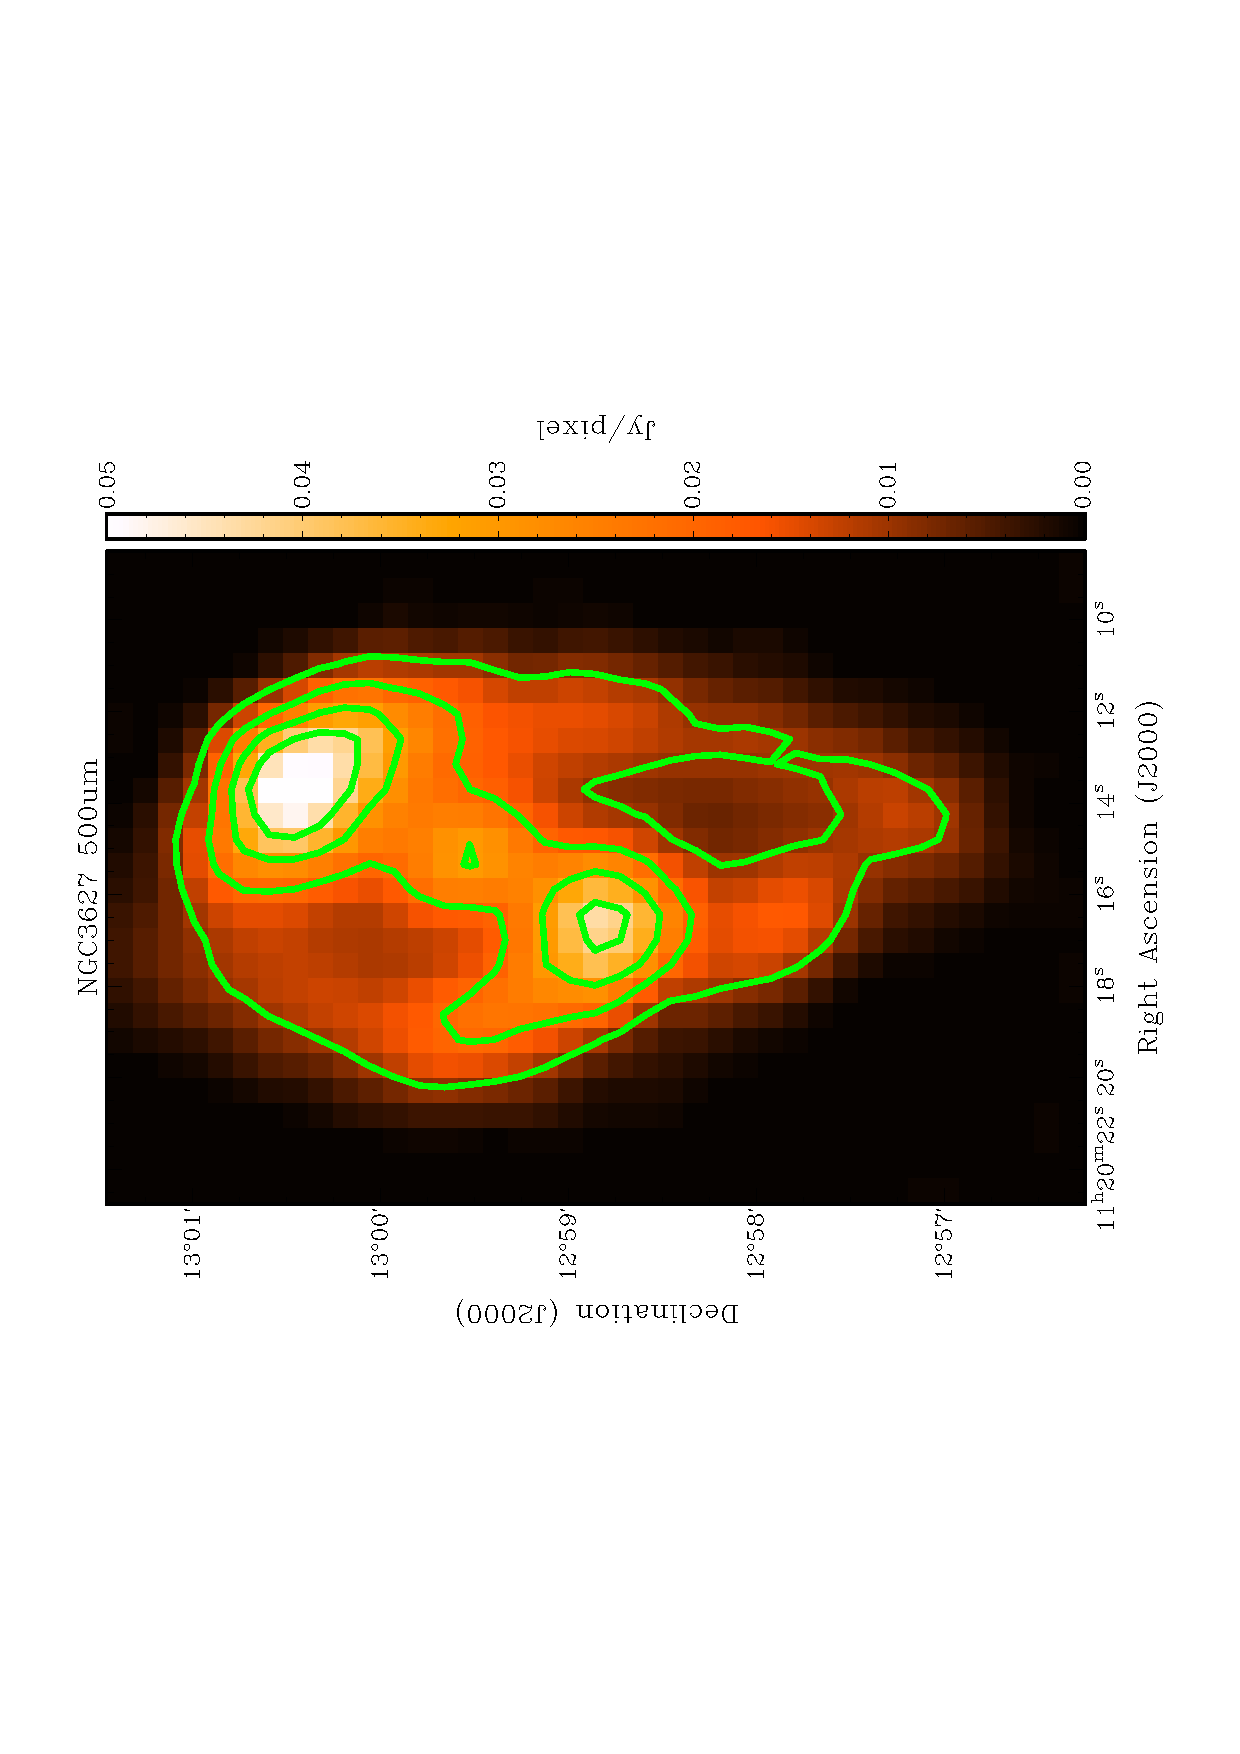
\includegraphics[scale=0.5,angle=270]{obs_imgs/500_um.jpeg}
  \caption[NGC3627 500$\mu$m Observations]{Residual of the MAKEMAP filtering of hte 500$\mu$m observations.}
\end{figure}

\begin{deluxetable}{cccc}
%  \tabletypesize{\footnotesize}
  \tablecolumns{4}
  \tablewidth{0pt}
  \tablecaption{Properties of NGC3627 KINGFISH Observations\label{tab_obs_kfish}}
  \tablehead{\colhead{Observation} & \colhead{Beam Properties } & \colhead{RMS} & \colhead{Percentage of Emission Removed} \\
 & $\theta_{beam}$ & \it{[Jy/Pixel]}}
  \startdata
    100$\mu$m & 6.8$\arcsec$ & 2.24e-3 & 16.7\% \\
    160$\mu$m & 11.6$\arcsec$ & 3.95e-3 & 18.8\% \\
    250$\mu$m & 18.0$\arcsec$ & 2.47e-3 & 19.9\% \\
    350$\mu$m & 24.9$\arcsec$ & 1.08e-3 & 21.8\% \\
    500$\mu$m & 36.0$\arcsec$ & 3.87e-4 & 27.7\% \\
  \enddata
\end{deluxetable}

\subsection{Nearby Galaxy Legacy Survey (NGLS)}

The Nearby Galaxy Legacy Survey is an HI-selected set of 155 galaxies contained in the annulus of $2Mpc\leq r \leq25Mpc$ using the instrumentation on the JCMT \citep{wilson2012}.  The NGLS consists of data observed in several wavelengths that include the 450$\mu$m and 850$\mu$m data used for this thesis.  As mentioned previously, the bandpass for SCUBA-2's 850$\mu$m emission contains the CO j=3-2 line which is contained in the NGLS data set.  We used the zeroth moment CO j=3-2 maps from the NGLS to determine the percentage of CO j=3-2 emission present in the 850$\mu$m band as well as removing it for an accurate SED analysis.  The rms and resolution of the CO j=3-2 emission are shown in table \ref{tab_obs_NGLS}, and the scan prior to convolution is shown in figure \ref{fig_co32}.

\begin{figure}
  \centering
  \label{fig_co32}
  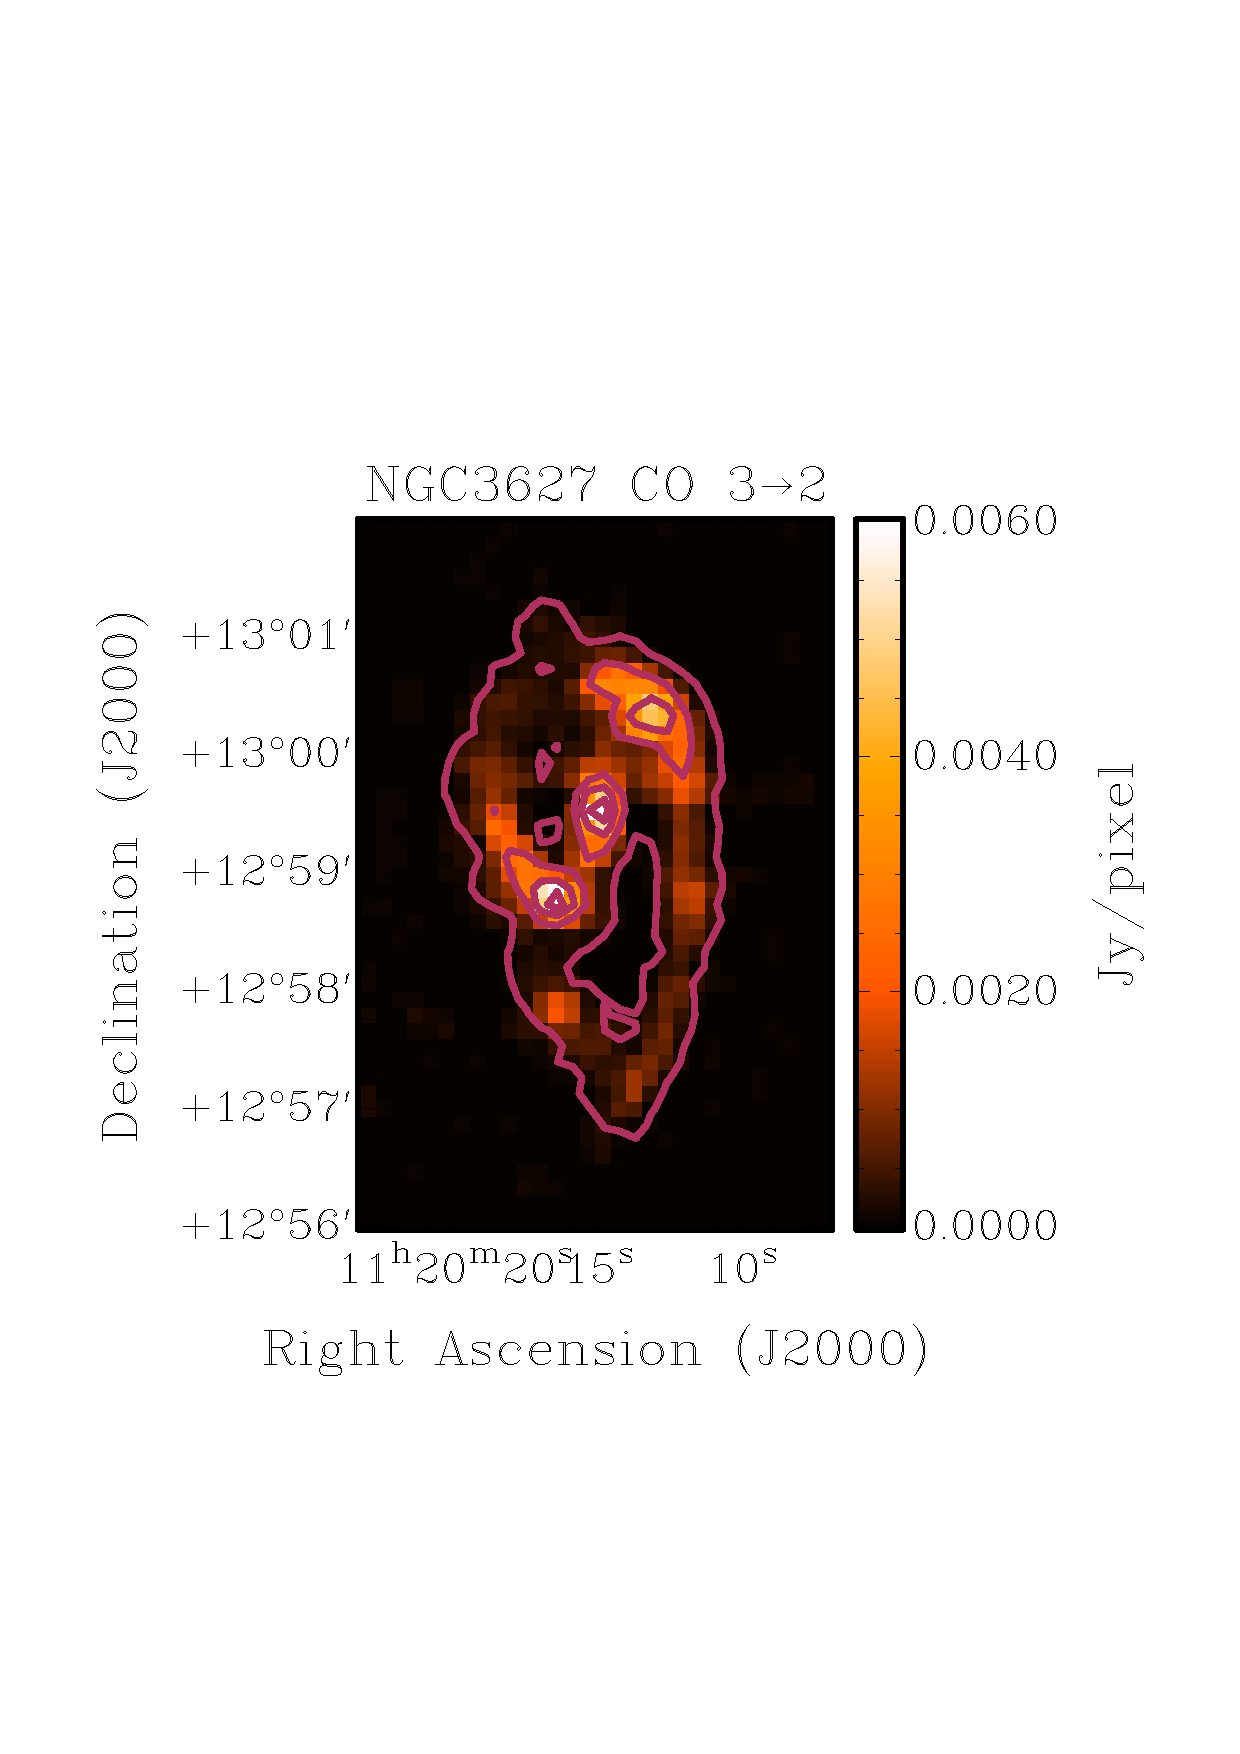
\includegraphics[scale=0.5]{obs_imgs/CO32.jpeg}
  \caption[NGC3627 CO j=3-2 Observations]{Residual of the MAKEMAP filtering of CO j=3-2 observations.}
\end{figure}

\begin{deluxetable}{cccc}
  \tablecolumns{4}
  \tablewidth{0pt}
  \tablecaption{Properties of NGC3627 NGLS Observations\label{tab_obs_NGLS}}
  \tablehead{\colhead{Observation} & \colhead{Beam Properties } & \colhead{RMS} & \colhead{Percentage of Emission Removed} \\
 & $\theta_{beam}$ & \it{[Jy/Pixel]}}
  \startdata
    CO j=3-2 & 14.5$\arcsec$ & 1.28e-5& 29.8\% \\
  \enddata
\end{deluxetable}

%insert co32 img

\subsection{Nobeyama 45-m}\label{nob_sec}

Determining a dust-to-gas ratio required the need for a molecular tracer to estimate the amount of molecular hydrogen present.  The most frequently used tracer is CO j=1-0 due to its abundance in the ISM.  The CO j=1-0 we used was taken from the Nobeyama 45-m CO Atlas of Nearby Spiral Galaxies observed to better understand the role of bars relating to molecular gas \citep{kuno2007}.  The Nobeyama 45-m CO Atlas consists of galaxies with morphologies ranging from Sa to Scd, located less that 25Mpc from the Milky Way, inclination values greater that $79^{\circ}$, 100$\mu$m flux greater than 10Jy, and spiral structure that has not be comprimised through interactions.  Any galaxies that met this criteria were then observed with the Nobeyama 45-m telescope \citep{kuno2007}  The beam sizes and rms of the filterd CO j=1-0 map are displayed in table \ref{tab_obs_n45} and the final image product can be seen in figure \ref{fig_co10}.

\begin{figure}
  \centering
  \label{fig_co10}
  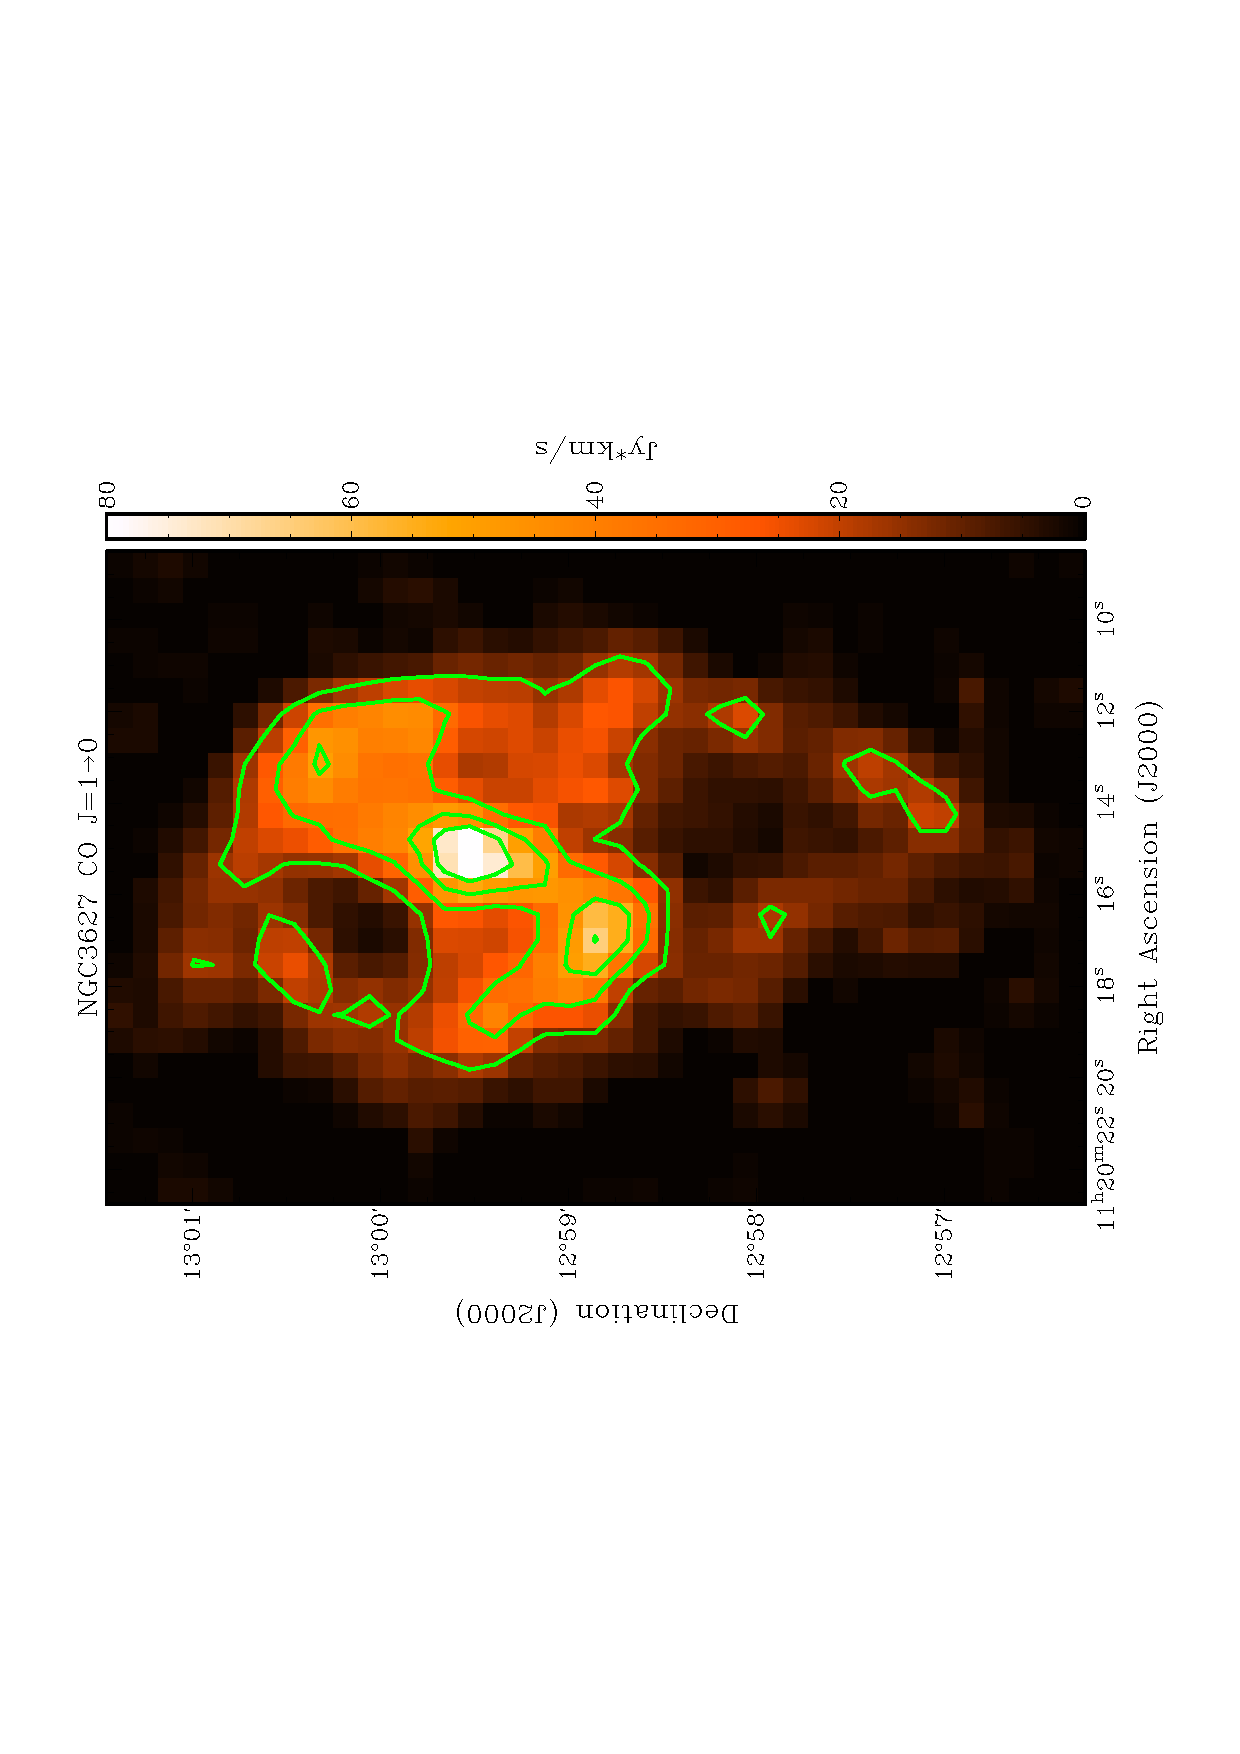
\includegraphics[scale=0.5]{obs_imgs/CO10.jpeg}
  \caption[NGC3627 CO j=1-0 Observations]{Residual of the MAKEMAP filtering of CO j=1-0 observations.}
\end{figure}

\begin{deluxetable}{cccc}
  \tablecolumns{4}
  \tablewidth{0pt}
  \tablecaption{Properties of NGC3627 Nobeyama 45-m Observations\label{tab_obs_n45}}
  \tablehead{\colhead{Observation} & \colhead{Beam Properties } & \colhead{RMS} & \colhead{Percentage of Emission Removed} \\ 
  & $\theta_{beam}$ & \it{[K km/s]}}
  \startdata
    CO j=1-0 & 15.0$\arcsec$ & 0.681 & 25.8\% \\
  \enddata
\end{deluxetable}

\subsection{Hetrodyne Reciever Array CO-Line Extragalactic Survey (HERACLES)}

The CO j=2-1 line was used to determine a ${2-1} / {1-0}$ line ratio which can be used to trace a gradient in $\alpha_{CO}$ and hint towards regions of high star-formation \citep{reuter1996}.  We used the CO j=1-0 data from the Nobeyama 45-m telescope ($\S$ \ref{nob_sec}), and CO j=2-1 from the Hetrodyne Reciever Array CO-Line Extragalactic Survey (HERACLES) using the IRAM 30-m telescope.  The main goal of HERACLES was to quantify the relationship between atomic and molecular gas and star formation using a large sample of galaxies (\citep{leroy2009}).  The sample of galaxies chosen were targets contained in THINGS that were within observing limits of the IRAM 30-m telescope.  The final image can be seen in figure \ref{fig_co21} and the image properties can be seen in table \ref{tab_obs_heracles}.

\begin{figure}
  \centering
  \label{fig_co21}
  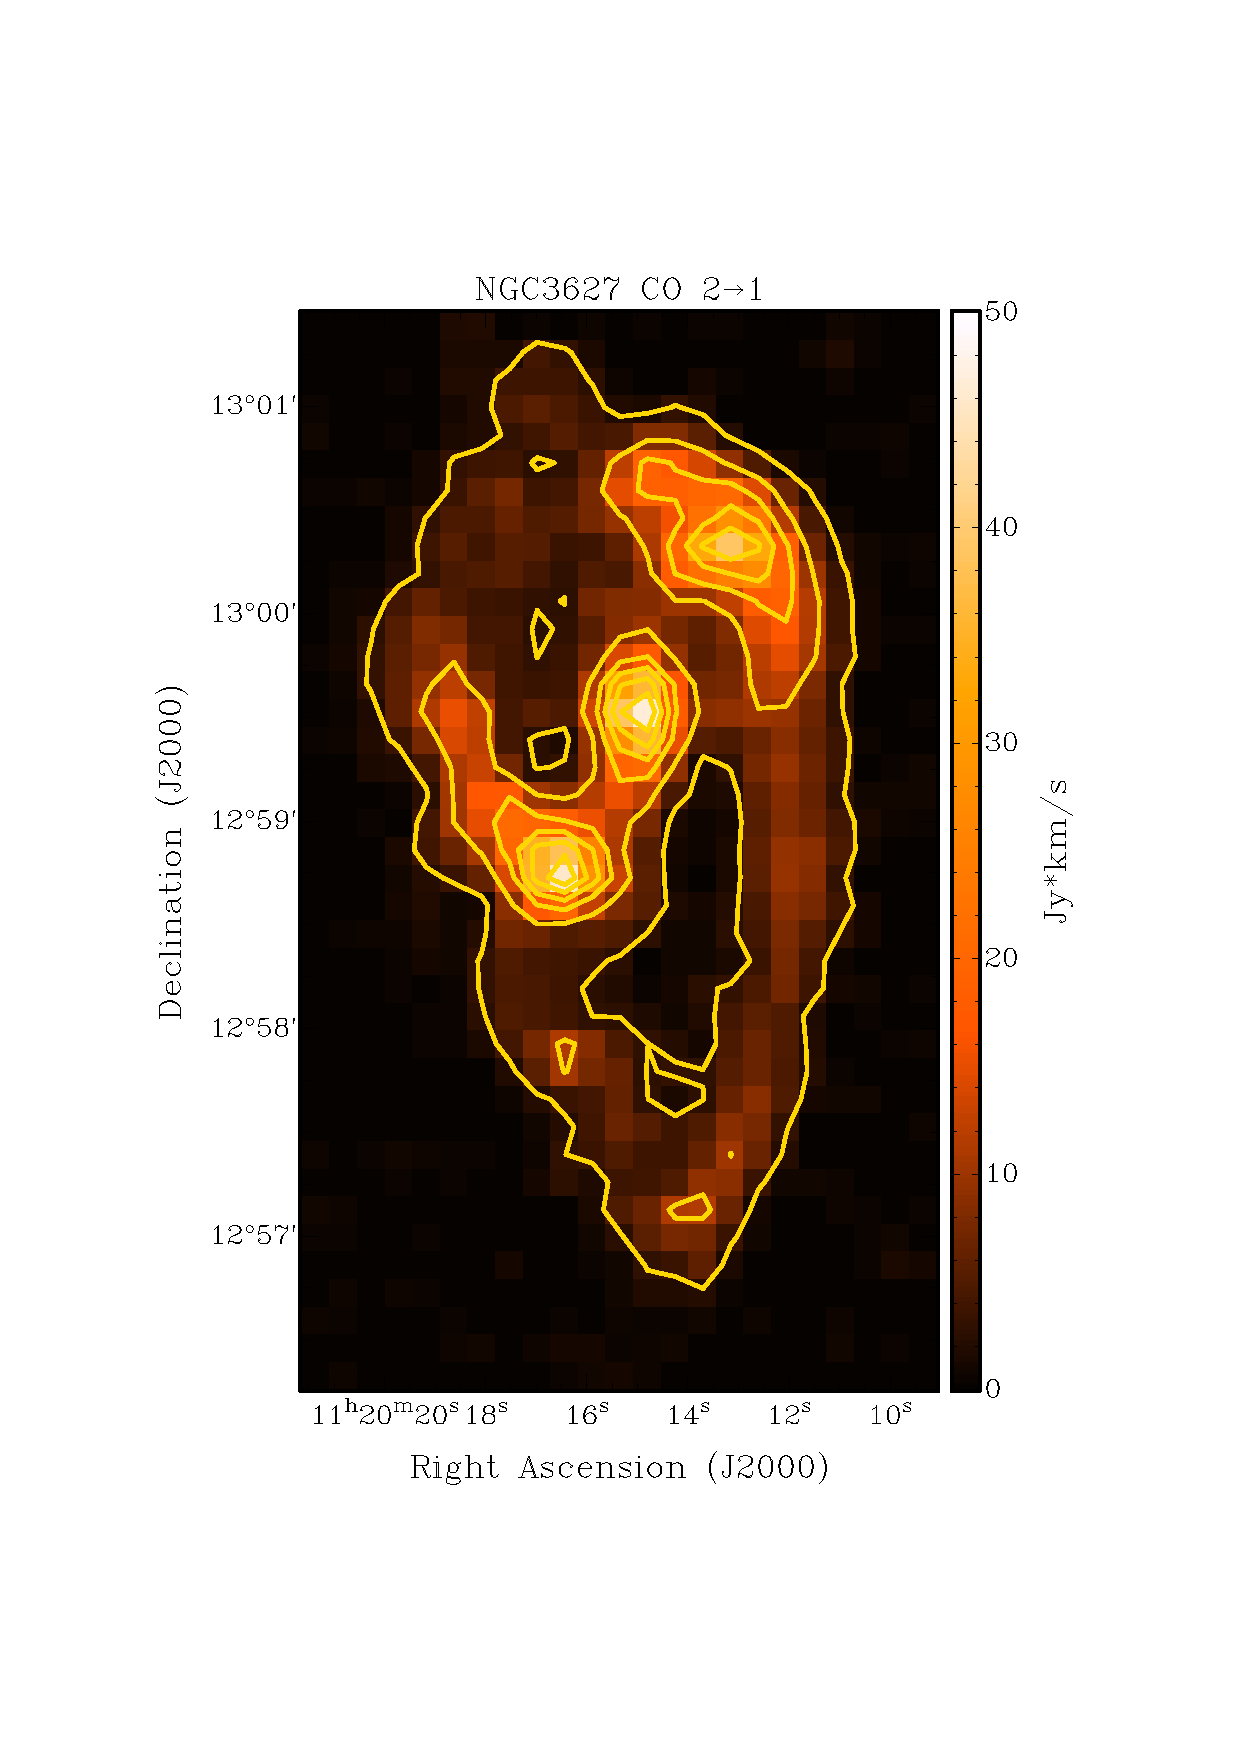
\includegraphics[scale=0.5]{obs_imgs/CO21.jpeg}
  \caption[NGC3627 CO j=2-1 Observations]{Residual of the MAKEMAP filtering of CO j=2-1 observations.}
\end{figure}

\begin{deluxetable}{cccc}
  \tablecolumns{4}
  \tablewidth{0pt}
  \tablecaption{Properties of NGC3627 HERACLES Observations\label{tab_obs_heracles}}
  \tablehead{\colhead{Observation} & \colhead{Beam Properties } & \colhead{RMS} & \colhead{Percentage of Emission Removed} \\
  & $\theta_{beam}$ & \it{[K km/s]}}
  \startdata
    CO j=2-1 & 13.0$\arcsec$ & 0.305 & 7.8\% \\
  \enddata
\end{deluxetable}

\subsection{The HI Nearby Galaxy Survey (THINGS)}

To determine the gas to dust ratio we had to determine the total amount of gas present which required both atomic and molecular hydrogen.  We approximated the amount of molecular hydrogen present by using CO j=1-0, and measured the amount of atomic hydrogen (HI) present.  The source of our atomic hydrogen came from The HI Nearby Galaxy Survey (THINGS) designed to observe HI emission in nearby galaxies with the extreme spatial resolution of the Very Large Array (VLA).  Targets in THINGS included many of the SINGS targets with the exception of known HI poor sources (E/S0 type galaxies), dynamicaly complex systems (edge-on spirals), and large extended galaxies found in the local group \citep{walter2008}.  The resolution and rms of the filtered image are shown in table \ref{tab_obs_things}.  The final data product is shown in figure \ref{fig_HI}.

\begin{figure}
  \centering
  \label{fig_HI}
  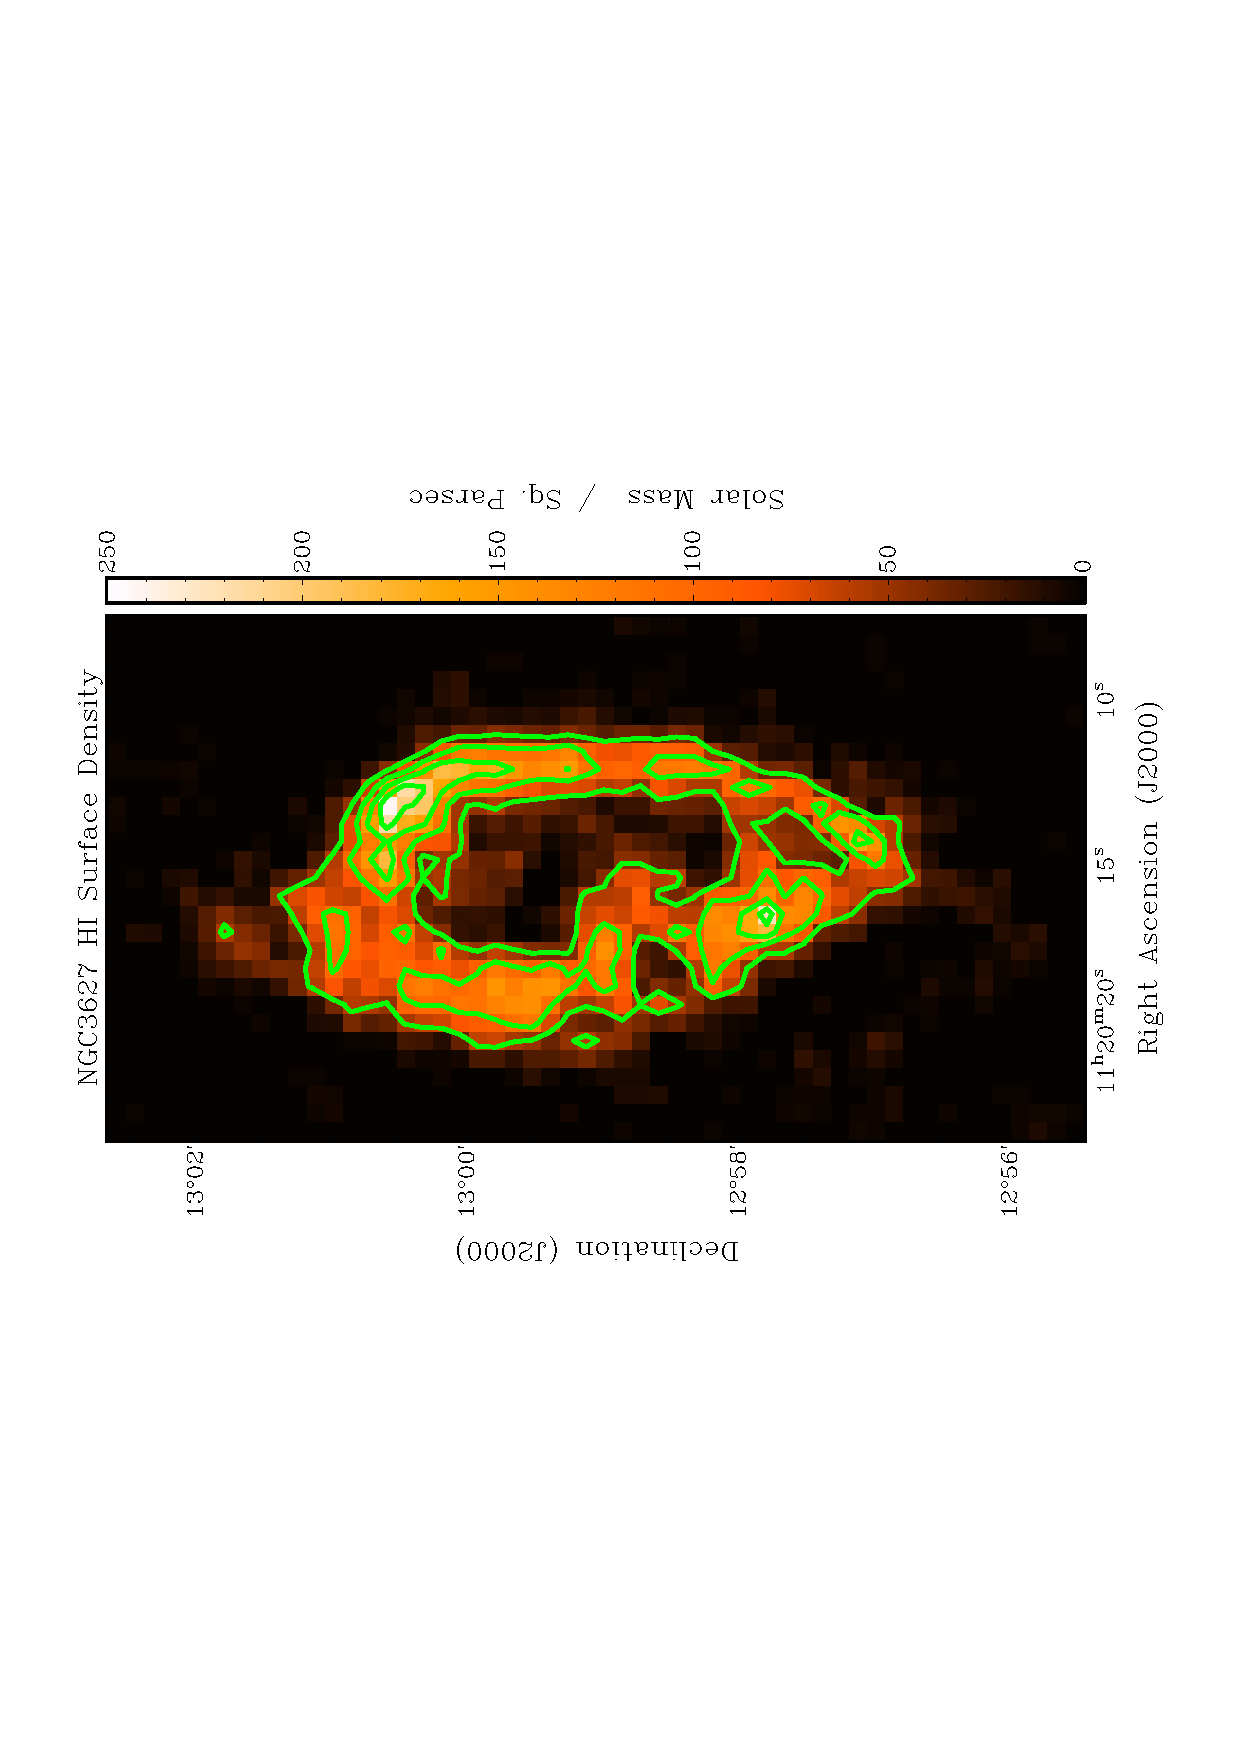
\includegraphics[scale=0.5,angle=270]{obs_imgs/HI.jpeg}
  \caption[NGC3627 HI Observations]{Residual of the MAKEMAP filtering of HI observations.}
\end{figure}

\begin{deluxetable}{cccccc}
  \tablecolumns{6}
  \tablewidth{0pt}
  \tablecaption{Properties of NGC3627 THINGS Observations\label{tab_obs_things}}
  \tablehead{\colhead{Observation} & \multicolumn{3}{c}{Beam Properties} & \colhead{RMS} & \colhead{Percentage of Emission Removed} \\
   & $\theta_{maj}$ & $\theta_{min}$ & $\theta_{PA}$ & \it{[$M_{\odot} / pc^2$]}}
  \startdata
    HI & 10.6$\arcsec$ & 8.85$\arcsec$ & -48.0$^\circ$ & 0.760 & 39.6\% \\  
  \enddata
\end{deluxetable}

\section{Data Preparation for Analysis}

Initially the data do not agree on several levels.  The differences consist of the presence of the large scale structure in some but not all of our maps, different resolutions, and accounting for the beam shape of the 450$\mu$m.  We have taken several steps to correct these disagreements and maximize the compatibility of the data.  In order to account for the varying beam resolutions, we use a gaussian convolution to increase the resolution of our maps to the largest beam size in our dataset, 36$\arcsec$, using equation \ref{eq:gaus_kern} to decide on an appropriate beam size such that $\sigma_{desire}$ is the desired beam width, $\sigma_{max}$ is the beam size we are convolving to, and $\sigma_{given}$ is the beams size we are convolving from.

\begin{equation}\label{eq:gaus_kern}
  \sigma_{desire} = \sqrt{\sigma_{max}^2 - \sigma_{given}^2}
\end{equation}

However, this only works when the beams are well approximated by a gaussian which is not the case for the 450$\mu$m beam.  The steps taken to match the resolution of the 450$\mu$m beam with the rest of the data set is given in $\S$ \ref{450_fix_sec}.  Removing any large scale structure from our ancillary data is implemented using a feature in MAKEMAP that allows us to add fake sources into the data during production.  The fake source implementation allows us to remove the same amount of large scale structure from our ancillary data as was removed from the SCUBA-2 data.  The steps taken to prepare the ancillary data are described in $S$\ref{fakesource_sec}.

%The largest difference in Ability of Herschell to observe submm unimpeded by atmo and the configuration setup of THIGNs allows for a bit of extended structure to arise in NGC3627.

\subsection{Accounting for the 450$\mu$m Error Beam}\label{450_fix_sec}

Taking the 450$\mu$m error beam into consideration is different than normal beam convolution in the sense that we are not convolving the higher resolution map to the lowest resolution.  Instead we are adding in an error beams similar to the 450$\mu$m observations to all of our observations.  We have to take these steps because convolving a double gaussian beam with a single gaussian kernel will not sufficiently remove the error component of our beam resulting in a poor approximation to the wings of our beam shape.

In order to accommodate the 450$\mu$m map's error beam, we used a method employed by another SCUBA-2 survey, the Gould-Belt Survey team.  This method used the distributive nature of the Fourier transform to create similar error components in the beam resolutions we were convolving to and from.  Carrying out this convolution involved breaking the 450$\mu$m beam into it's two components, $\sigma_{\alpha}$ and $\sigma_{\beta}$ to represent the main beam and error beam.  The lowest resolution beam shape, $\sigma_{max}$ is convolved with the two components and the resulting beams are added together.  This process produces an equivalent two component beam as the 450$\mu$m beam conolved with $\sigma_{max}$.  This relationship is shown in equation \ref{eq_GBSmethod} where $X_{max}$ is the beam width of the our lowest resolution, $X_{\alpha}$ and $X_{\beta}$ are the main and error beam of the 450$\mu$m observations, and $X_{450\mu m}$ is the double gaussian beam shape of the 450$\mu$m observations.

\begin{equation} \label{eq_GBSmethod}
  X_{max} \ast X_{\alpha} + X_{max} \ast X_{\beta} = \left(X_{\alpha} + X_{\beta}\right) \ast X_{max} = X_{450\mu m} \ast X_{max}
\end{equation}

\subsection{Extended Structure Removal via MAKEMAP}\label{fakesource_sec}

%adjusting the beam sizes to make the 450 beam work

%from the ancillary data set -- describes the fakesource stuff
Due to the combination of methods used in MAKEMAP, small scale/extended structure is removed from the final SCUBA-2 images.  However, in all of our ancillary data the small scale emission was present in the initial maps.  The removal of the extended features from our support data was carried out by either converting the images from their native units into pW using the 850$\mu$m flux calibration factor or by introducing a scaling factor.  The images were overlaid on the original scans as a fakesource and passed through the reduction process.  The original scan was then subtracted from the scan with the fakesource present and the residual of the process was the ancillary data with its extended structure removed.

%KINGFISH filtering
We were interested in fitting the cold component of NGC3627's SED, hence we omitted the 70$\mu$m emission, and used the 100$\mu$m, 160$\mu$m, 250$\mu$m, 350$\mu$m and 500$\mu$m.  Since the Kingfish data was acquired by a space-based telescope, a significant amount of small scale emission was recovered due to the lack of interference from the atmosphere.  The small scale emission was removed by treating the KINGFISH data as a fakesource in the image reduction process.  The first step to successfully incorporating the data as a fakesource was to convert the 250$\mu$m, 350$\mu$m, and 500$\mu$m from MJy/sr to mJy/square arcsecond, and similarly the 100$\mu$m and 160$\mu$m from Jy/pixel to mJy/square arcsecond.   After the unit conversion, the 850$\mu$m flux calibration factor was applied in reverse, and the new image was then scaled down to better mimic the 850$\mu$m emission.  After these steps the image was passed into MAKEMAP and treated as an 850$\mu$m image.  The final data output were gridded to 8$\arcsec$ x 8$\arcsec$ pixels correspoding to a 20kpc scale.  The outputted images can be seen in figures \ref{fig_100} through \ref{fig_500}.  The beam size and rms for each image after it has been passed through make map can be seen in table \ref{tab_obs_kfish}.

%NGLS processing
Removing the CO j=3-2 contamination from the 850$\mu$m images required passing the data through MAKEMAP in a similar manner as the KINGFISH data.  The only significant difference was converting the CO j=3-2 data from $K*km/s$ to pW.  The change of units was done using conversion factor of 0.70 $[K*km/s][mJy/beam]^{-1}$ found by \citep{drabek2012} for the task of converting HARP observations to the same units as SCUBA-2 850$\mu$m data.  The final image product can be seen in figure \ref{fig_co32}.  We found the average ratio of CO j=3-2 to 850$\mu$m to be around 29\% with some regions dropping to less than 6\%.  The amount of flux removed and the filtered image's rms can be found in table \ref{tab_obs_NGLS}.

%NOB processing
Preparation for the CO j=1-0 was performed in a similar matter to the previous ancillary data sets, however instead of determining a direct conversion factor the zeroth moment map was scaled down by a factor 0.001.  The scaling factor used was used in lieu of the unit conversion method so the final image would be in it's native units of ($K km/s$) at the end of filtering.  The scaling factor was determined in a way such that the input image for the fakesoure would be on the same order of magnitude as the 850$\mu$m image it was being added onto.  The scaling factor was then re-applied as the flux calibration factor to return the filtered map to its original magnitude.

%HERACLES processing
The HERACLES data was treated in the same manner as the Nobeyama 45-m when filtering was applied.  Since both the CO j=1-0 and CO j=2-1 were on the same order of magnitude, the same scaling factor of 0.001 was applied before and after the filtering.

%THINGS processing

The preparation of the HI data was similar to the $CO$ filtering in the sense we did not convert the image into pW and let it remain in its native units.  The major difference in the HI extended emission filtering was we did not use a flux map for the final processing; instead we used a surface density map as our fakesource.  This was due to issues that arose when using the mass formula given in \citep{walter2008} on a filtered image.  Due to the high resolution of the VLA we measured significant losses in flux due to small scale structure after filtering.  The amount of lost structure for NGC3627 as a whole can be seen intable 
